\documentclass[12pt,twoside,openright]{book}

% --- Codifica e lingua ---
\usepackage[utf8]{inputenc}
\usepackage[T1]{fontenc}
\usepackage{lmodern}
\usepackage[italian]{babel}

% --- Matematica ---
\usepackage{amsmath}
\usepackage{amssymb}
\usepackage{amsfonts}
\usepackage{etoolbox}

% --- Colori e grafica ---
\usepackage{xcolor}
\usepackage{graphicx}
\usepackage{subcaption}
\usepackage{float}

\usepackage{tikz}
\usetikzlibrary{shapes.geometric, arrows.meta}

% --- Layout pagina ---
\usepackage[a4paper, margin=2.8cm, bindingoffset=1cm]{geometry}
\usepackage[expansion=false]{microtype}
\usepackage{fancyhdr}
\usepackage{titlesec}
\usepackage{emptypage}
\usepackage{placeins}

% --- Tabelle e unità di misura ---
\usepackage{booktabs}
\usepackage{siunitx}
\usepackage{tabularx}

% --- Algoritmi e codice ---
\usepackage[ruled,vlined]{algorithm2e}
\usepackage{listings}

% --- tcolorbox per teoremi/definizioni/esempi ---
\usepackage[most]{tcolorbox}
\tcbuselibrary{theorems}

% --- Hyperref: va caricato quasi per ultimo ---
\usepackage[colorlinks=true, linkcolor=black, citecolor=black, urlcolor=blue]{hyperref}

% ============================================================
% Colore principale della tesi
% ============================================================
\definecolor{accento}{RGB}{30,80,30} % verde scuro

% ============================================================
% tcolorbox: esempio, dimostrazione, teorema
% ============================================================
\newtcbtheorem[number within=section]{example}{Esempio}%
  {colback=accento!5, colframe=accento, fonttitle=\bfseries}{ex}

\newtcbtheorem[number within=section]{dimost}{Dimostrazione}%
  {colback=accento!8, colframe=accento, fonttitle=\bfseries, coltitle=white}{def}

\newtcbtheorem[number within=section]{theorem}{Teorema}%
  {colback=accento!10, colframe=accento, fonttitle=\bfseries, coltitle=white,
   colbacktitle=accento}{thm}

% ============================================================
% Formattazione capitoli
% "Capitolo N" ora sopra le due righe, e più grande (\Huge)
% ============================================================
\titleformat{\chapter}[display]
{\normalfont\filcenter}
{\textcolor{accento}{\Huge\textsc{\chaptertitlename\ \thechapter}}
 \vspace{1ex}
 \titlerule[1 pt]\vspace{1pt}\titlerule}
{1ex}
{\centering\Huge\bfseries}

\titlespacing*{\chapter}{0pt}{40pt}{15pt}
\titlespacing*{\section}{0pt}{*2}{*1}

% ============================================================
% Intestazioni/piè di pagina
% ============================================================
\pagestyle{fancy}
\setlength{\headheight}{14.5pt}
\fancyhf{}
\fancyhead[LE,RO]{\thepage}
\fancyhead[RE]{\nouppercase{\leftmark}}
\fancyhead[LO]{\nouppercase{\rightmark}}
\renewcommand{\headrulewidth}{0.4pt}

\fancypagestyle{plain}{%
  \fancyhf{}
  \fancyhead[LE,RO]{\thepage}
  \renewcommand{\headrulewidth}{0pt}
}

% Profondità indice / numerazione sezioni
\setcounter{tocdepth}{2}
\setcounter{secnumdepth}{3}

% ============================================================
% Pagina bianca "vera" prima di ogni capitolo
% openright + \cleardoublepage inseriscono già una pagina vuota
% quando serve, ma di default mostrano comunque il numero di
% pagina nell'intestazione. Questa ridefinizione forza lo stile
% "empty" (nessun numero, nessuna intestazione) su quella pagina.
% ============================================================
\makeatletter
\renewcommand{\cleardoublepage}{%
  \clearpage
  \if@twoside
    \ifodd\c@page\else
      \hbox{}
      \thispagestyle{plain}
      \newpage
      \if@twocolumn\hbox{}\newpage\fi
    \fi
  \fi
}
\makeatother

% Comando comodo per pagine bianche (stesso trattamento delle pagine
% bianche automatiche prima dei capitoli: stile "plain", solo numero
% di pagina, nessuna intestazione testuale)
\newcommand{\blankpage}{\newpage\thispagestyle{plain}\null\newpage}

\begin{document}

% ============================================================
% FRONTESPIZIO
% ============================================================
\begin{titlepage}
\begin{center}
\resizebox{\textwidth}{!}{\textsc{Alma Mater Studiorum $\cdot$ Universit\`a di Bologna}}
\rule[0.1cm]{\textwidth}{0.1mm}
\rule[0.5cm]{\textwidth}{0.6mm}
\\\vspace{3mm}

{\small{\bf Dipartimento di Fisica e Astronomia “Augusto Righi”\\
Corso di Laurea in Fisica}}

\end{center}

\vspace{23mm}

\begin{center}
\begin{minipage}{0.85\textwidth}
\centering
{\LARGE\bfseries\linespread{1.15}\selectfont
Metodi Monte Carlo e Normalizing Flows generativi per il campionamento di distribuzioni di Boltzmann multimodali\par}
\end{minipage}
\end{center}

\vspace{50mm} \par \noindent

\begin{minipage}[t]{0.47\textwidth}

{\large{\bf Relatore: \vspace{2mm}\\\textcolor{black}{
Prof. Cesare Franchini}\\\\
\textcolor{black}{
\bf Correlatore:
\vspace{2mm}\\
Dott. Luca Leoni\\\\}}}
\end{minipage}
%
\hfill
%
\begin{minipage}[t]{0.47\textwidth}\raggedleft \textcolor{black}{
{\large{\bf Presentata da:
\vspace{2mm}\\
Riccardo Pivi}}}
\end{minipage}

\vfill

\begin{center}
Anno Accademico \textcolor{black}{ 2025/2026}
\end{center}
\end{titlepage}

\pagenumbering{gobble} 

\blankpage

% --- Dedica ---
\vspace*{90mm}
\begin{flushright}
\itshape
A mio fratello e ai miei genitori,\\
per essere stati il mio faro\\ e il mio porto sicuro.
\end{flushright}
\vspace*{\fill}

\cleardoublepage

\begin{center}
    {\LARGE\bfseries Sommario}
\end{center}

\vspace{1cm}

Il calcolo delle proprietà macroscopiche di un sistema fisico a partire dalla sua descrizione microscopica richiede, nell'ambito della meccanica statistica, la valutazione di valori di aspettazione rispetto alla distribuzione di Boltzmann. Poiché lo spazio delle configurazioni ha dimensione pari al numero di gradi di libertà del sistema, tale calcolo è generalmente inaccessibile per via analitica o mediante integrazione numerica, ed è affrontato tramite metodi Monte Carlo, che sostituiscono il calcolo esatto con una stima statistica basata sul campionamento.
 
Un metodo di campionamento a cui si ricorre è \emph{Markov Chain Monte Carlo} (MCMC), tipicamente utilizzato con proposte locali. Per quanto generale, questo approccio mostra un limite intrinseco quando la distribuzione target è multimodale: ovvero quando presenta modi di alta densità separati da regioni a bassa densità di probabilità. In questo caso la catena di Markov può rimanere intrappolata in un singolo modo per tempi computazionali proibitivi, compromettendo il corretto capionamento (fenomeno noto come \emph{intrappolamento nei modi}).
 
Questa tesi esplora una strategia alternativa basata sui \emph{Normalizing Flows} (NF), una classe di modelli generativi costruiti tramite trasformazioni invertibili e differenziabili. Un NF addestrato ad approssimare la distribuzione di Boltzmann può essere impiegato in due modi: come motore di campionamento diretto, le cui stime vengono poi corrette tramite \emph{importance sampling}; oppure come distribuzione di proposta globale all'interno di in un metodo ibrido (Flow-MCMC), che unisce la capacità di esplorazione globale del Normalizing Flow alla correttezza asintotica garantita da Markov Chain Monte Carlo.

I tre metodi - MCMC, NF e Flow-MCMC - vengono confrontati empiricamente su un sistema di test a potenziale doppio pozzo, scelto per la bimodalità che induce alla distribuzione di Boltzmann. Si quantifica l'efficienza del campionamento al variare della temperatura e del numero di campioni. I risultati mostrano che, a basse temperature, l'MCMC locale rimane sistematicamente confinato in un solo pozzo del potenziale, producendo stime distorte. NF e Flow-MCMC, al contrario, mantengono un'esplorazione bilanciata dei due modi e una convergenza più rapida su tutto l'intervallo di temperature considerato, confermando l'assenza di intrappolamento nei modi e dunque il vantaggio pratico delle mosse globali basate sui Normalizing Flows rispetto al campionamento markoviano locale in presenza di distribuzioni di probabilità multimodali.

\cleardoublepage

\tableofcontents

% ============================================================
% Main matter: numerazione araba da qui
% ============================================================
\pagenumbering{arabic}
\pagestyle{fancy} 
\setcounter{page}{1}

\chapter*{Introduzione}
\addcontentsline{toc}{chapter}{Introduzione}

\chapter{Probabilità e meccanica statistica}
In questo capitolo vengono introdotti alcuni concetti fondamentali di probabilità necessari per comprendere il problema del campionamento: esso consiste nel generare una successione di configurazioni secondo una determinata distribuzione di probabilità. Tale problema assume particolare rilevanza in meccanica statistica, dove le proprietà macroscopiche di un sistema possono essere ricavate a partire dalle configurazioni microscopiche che lo costituiscono.

Dopo aver introdotto le nozioni di base relative alle variabili aleatorie e alle distribuzioni di probabilità, si discuterà l'importanza del campionamento di una distribuzione. Infine, si introdurrà l'ensemble canonico, con particolare attenzione alla distribuzione di Boltzmann, che rappresenta la distribuzione target dei metodi di campionamento studiati nel seguito di questa tesi.

\section{Teoria della probabilità}
\subsection{Spazi di probabilità e variabili aleatorie}
In teoria della probabilità ha un ruolo fondamentale \textbf{lo spazio di probabilità} ($ \Omega, P$): dove $\Omega$ è l'insieme di tutti i possibili eventi $\chi$ e $P$ è una misura di probabilità su $\Omega$. Un sottoinsieme $A \subset \Omega$ è chiamato evento ed ad ogni evento è possibile associare un numero reale $P(A) \in [0, 1]$ - ovvero la probabilità di tale evento. In particolare è necessario che sia soddisfatte $P(\Omega) = 1$, $ P(\emptyset) = 0$ e per ogni insieme di eventi disgiunti $A_1, A_2,  ...$ vale:

\begin{equation}
    P(A_1 \cup A_2 \ ...) = P(A_1) + P(A_2) + ...
\end{equation}

\begin{example}{Tiri di un dado}{dice}
Quando si tira un dado a sei facce si considera lo spazio degli eventi $\Omega = \{1, 2, ... , 6\}$ e la misura di probabilità $P({\chi_i}) = 1/6$ per ogni $\chi_i \in \Omega$ .
Un esempio di evento è il caso in cui risultato del tiro sia pari $A =\{2, 4, 6\} \subset \Omega$ con probabilià calcolabile nel seguente modo: $P(A) = P({1}) + P({2}) + P({3}) = 1/2$.
\end{example}


Una \textbf{variabile aleatoria} (reale) $X$ che associa agli elementi di uno spazio degli esiti $\Omega$ valori appartenenti a uno spazio misurabile $(\mathbb{R})$. 
Una variabile aleatoria $X$ associa a ciascun esito $\chi$ un valore $x$ appartenente allo spazio dei valori possibili della variabile. Nel caso di una variabile aleatoria reale si ha quindi:
\begin{equation}
X:\Omega \rightarrow \mathbb{R}.
\end{equation}

\subsection{Distribuzioni di probabilità continue}

La distribuzione di probabilità associata a una variabile aleatoria continua $X$ è descritta da una densità di probabilità $p_X(x)$, che determina come la probabilità è distribuita nello spazio dei possibili valori di $X$. La densità di probabilità deve soddisfare la condizione di normalizzazione
\begin{equation}
\int_{-\infty}^{+\infty}p_X(x) \ dx=1.
\end{equation}

È importante sottolineare che, nel caso continuo, la densità di probabilità non rappresenta direttamente la probabilità che la variabile assuma un determinato valore. Infatti, la probabilità di ottenere esattamente un particolare valore $x_0$ è nulla. La densità di probabilità permette invece di calcolare la probabilità che la variabile aleatoria assuma un valore appartenente a un determinato intervallo. In particolare, la probabilità che $X$ appartenga all'intervallo $[a,b]$ è data da
\begin{equation}
P(a\leq X\leq b)
=
\int_a^b p_X(x) dx.
\end{equation}

La distribuzione di probabilità può quindi essere interpretata geometricamente: la probabilità associata a un intervallo corrisponde all'area sottesa dalla densità di probabilità nell'intervallo considerato. Una maggiore densità di probabilità in una determinata regione indica quindi una maggiore probabilità di osservare valori della variabile in quella regione.

Nel seguito sarà particolarmente utile considerare variabili aleatorie multidimensionali. Una configurazione microscopica di un sistema fisico può infatti essere rappresentata mediante un vettore
\begin{equation}
\mathbf{x}=(x_1,x_2,\ldots,x_D)\in\mathbb{R}^D,
\end{equation}
dove $D$ rappresenta il numero di gradi di libertà del sistema. In questo caso la distribuzione di probabilità è descritta da una densità $p(\mathbf{x})$, normalizzata secondo
\begin{equation}
\int_{\mathbb{R}^D}p(\mathbf{x})d\mathbf{x}=1.
\end{equation}

La densità $p(\mathbf{x})$ permette di determinare la probabilità che una configurazione appartenga a una determinata regione $\mathcal{A}$ dello spazio delle configurazioni:
\begin{equation}
P(\mathbf{x}\in\mathcal{A})
=
\int_{\mathcal{A}}p(\mathbf{x}) \ d\mathbf{x}.
\end{equation}

Nel caso multidimensionale la probabilità è l'integrale della densità di probabilità su una regione dello spazio delle configurazioni. Analogamente al caso unidimensionale, non è la probabilità associata a una singola configurazione a essere rilevante, ma la probabilità complessiva associata a una regione dello spazio.

Una distribuzione di probabilità può inoltre presentare una struttura caratterizzata dalla presenza di uno o più massimi locali. In particolare, si definisce distribuzione \textit{unimodale} una distribuzione caratterizzata da un'unica regione di massima probabilità detta \textit{modo}. Un esempio tipico è rappresentato dalla distribuzione gaussiana, che presenta un unico massimo in corrispondenza del suo valore medio.

Una distribuzione \textit{multimodale}, invece, presenta più regioni distinte di alta probabilità, associate a più massimi locali della densità. In questo caso, ciascun massimo identifica un modo della distribuzione. Le diverse regioni ad alta probabilità possono essere separate da regioni caratterizzate da una densità molto più bassa.

\begin{figure}[H]
    \centering
    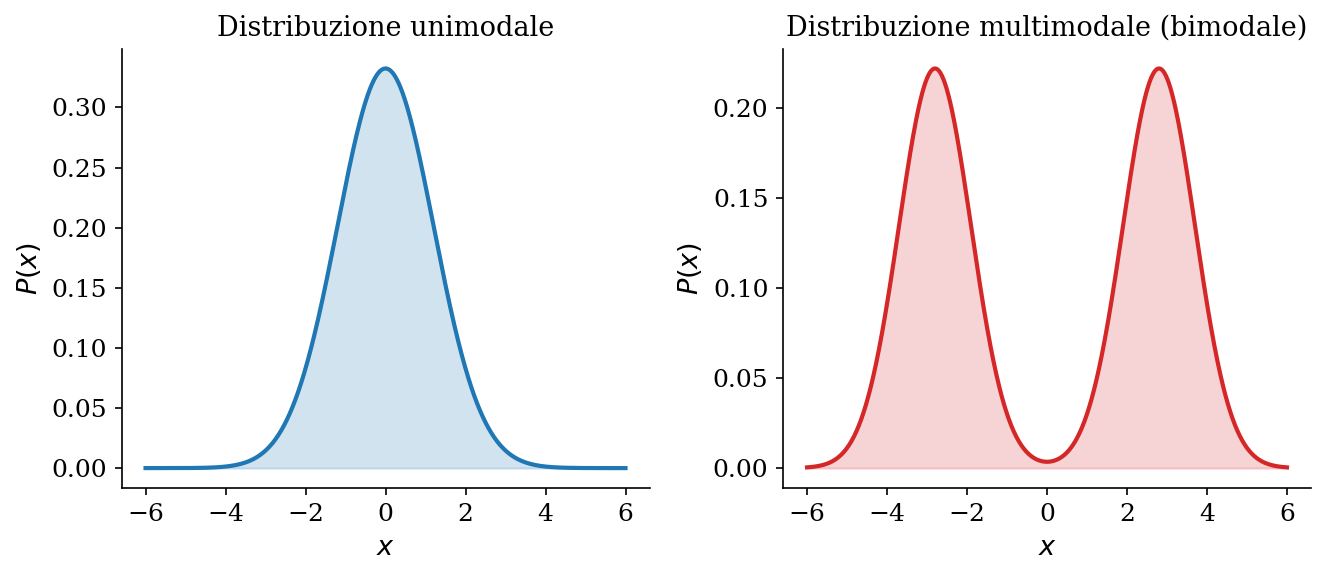
\includegraphics[width=0.9\textwidth]{images/uni_multi.png}
    \caption{Confronto tra una distribuzione unimodale (gaussiana) e una distribuzione multimodale (bimodale).}
    \label{fig:uni_multi}
\end{figure}

La distinzione tra distribuzioni unimodali e multimodali è particolarmente importante nel problema del campionamento. Nel caso di una distribuzione unimodale, un metodo di campionamento che esplori efficacemente la regione attorno al massimo della distribuzione può ottenere un campione rappresentativo dell'intera distribuzione. Nel caso multimodale, invece, il campionamento può risultare più complesso, poiché è necessario esplorare tutte le regioni rilevanti dello spazio delle configurazioni e riprodurre correttamente la probabilità associata a ciascun modo e non esclusivamente a quello di maggiore densità.

Se le diverse regioni ad alta probabilità sono separate da barriere caratterizzate da una probabilità molto bassa, un metodo di campionamento locale può infatti rimanere confinato per lungo tempo all'interno di uno dei modi, esplorando con difficoltà gli altri. Questo fenomeno rappresenta una delle principali difficoltà associate al campionamento di distribuzioni multimodali e costituisce uno degli aspetti centrali affrontati nel seguito della tesi.

\subsection{Valori di aspettazione e campionamento}

Sia $O(\mathbf{x})$ una funzione della variabile aleatoria, il valore di aspettazione è calcolabile tramite il seguente integrale:

\begin{equation}
\langle O(\mathbf{x})\rangle
=
\int_{\mathbb{R}^D} O(\mathbf{x})p(\mathbf{x}) \ d\mathbf{x}.
\end{equation}

La convergenza dell'integrale non è affatto garantita e dipende dall'andamento della funzione $O(\mathbf{x})$ e da $p(\mathbf{x})$, inoltre questo integrale non è sempre facilemente risolvibile analiticamente o numericamente.
Un approccio diretto al calcolo di $\langle O(\mathbf{x})\rangle$ potrebbe basarsi su metodi di quadratura numerica, che discretizzano lo spazio delle configurazioni su una griglia e approssimano l'integrale come somma pesata sui punti della griglia. Se lo spazio delle configurazioni ha dimensione $D$ e si utilizzano $n$ punti per ciascuna direzione, il numero totale di valutazioni della funzione integranda cresce come $n^D$. Per sistemi con un numero elevato di gradi di libertà, come tipicamente accade in meccanica statistica, questa crescita esponenziale rende i metodi di quadratura del tutto inapplicabili: questo fenomeno è noto come \textit{maledizione della dimensionalità}.

È in questo contesto che il campionamento assume un ruolo centrale. Anziché valutare la funzione integranda su una griglia deterministica, l'idea alla base dei metodi di campionamento consiste nel generare un insieme di configurazioni $\{\mathbf{x}_1,\mathbf{x}_2,\ldots,\mathbf{x}_N\}$ distribuite secondo la densità di probabilità $p(\mathbf{x})$, e nello stimare il valore di aspettazione mediante la media aritmetica
\begin{equation}
\langle O(\mathbf{x})\rangle
\approx
\overline{O}_N
=
\frac{1}{N}\sum_{i=1}^{N}O(\mathbf{x}_i).
\label{eq:mc_estimator}
\end{equation}

Per la legge dei grandi numeri, lo stimatore $\overline{O}_N$ converge, per $N\rightarrow\infty$, al valore di aspettazione esatto $\langle O(\mathbf{x})\rangle$, a patto che le configurazioni $\mathbf{x}_i$ siano effettivamente distribuite secondo $p(\mathbf{x})$. Un aspetto cruciale di questo approccio è che, se le configurazioni sono indipendenti e identicamente distribuite, l'errore statistico associato allo stimatore decresce come
\begin{equation}
\sigma_{\overline{O}_N} \sim \frac{\sigma_O}{\sqrt{N}},
\end{equation}
dove $\sigma_O$ è la deviazione standard di $O(\mathbf{x})$ rispetto a $p(\mathbf{x})$. Diversamente dai metodi di quadratura, questo risultato non dipende esplicitamente dalla dimensione $D$ dello spazio delle configurazioni: è questa caratteristica a rendere i metodi di campionamento lo strumento privilegiato per lo studio di sistemi ad alta dimensionalità. Il problema del campionamento, in questo senso, precede logicamente quello della stima delle osservabili, e sarà l'oggetto centrale dei metodi discussi nei capitoli successivi.

\section{Ensemble statistici}



\subsection{L'ensemble canonico}
Consideriamo un sistema fisico descritto da una hamiltoniana $\mathcal{H}(\mathbf{x})$ dove $\mathbf{x}$
rappresenta collettivamente i gradi di libertà del sistema: posizioni, impulsi, o in generale le variabili che definiscono uno stato microscopico. L'ensemble canonico permette di descrivere il comportamento termodinamico di un sistema posto a contatto termico con un \textit{reservoir}  a temperatura $T$ fissata, con cui può scambiare energia ma non particelle. L'energia del sistema fluttua attorno a un valore medio $\langle E \rangle$ determinato dall'equilibrio termico con il serbatoio.

\subsection{La distribuzione di Boltzmann}


Il comportamento del sistema a fissata $T$ è descritto da una distribuzione di probabilità $\rho (\mathbf{x}, T)$ ottenibile attraverso il principio di massima entropia.
\begin{equation}
    \mathcal{S} = - \int_{\mathbb{R}^D} \rho (\mathbf{x}, T) \ln(\rho(\mathbf{x}, T)) d\mathbf{x}
\end{equation}

Per massimizzare l'entropia si utilizza il teorema dei moltiplicatori di Lagrange:

\begin{equation}
    \mathcal{L}[\rho] = -\int_{\mathbb{R}^D} \rho \ln \rho \, d\mathbf{x} - \alpha \left( \int_{\mathbb{R}^D} \rho \, d\mathbf{x} - 1 \right) - \beta \left( \int_{\mathbb{R}^D} \rho \, \mathcal{H} \, d\mathbf{x} - \langle E \rangle \right),
\end{equation}

dove $\alpha$ e $\beta$ sono i moltiplicatori di Lagrange associati rispettivamente al vincolo di normalizzazione

\begin{equation}
    \int_{\mathbb{R}^D} \rho(\mathbf{x}, T) \ d\mathbf{x} = 1
\end{equation}

e al vincolo sul valore medio dell'energia

\begin{equation}
    \int_{\mathbb{R}^D} \rho(\mathbf{x}, T) \, \mathcal{H}(\mathbf{x}) \, d\mathbf{x} = \langle E \rangle .
\end{equation}

La massimizzazione impone $\delta \mathcal{L}/\delta \rho = 0$ restituendo:

\begin{equation}
    -\ln\rho(\mathbf{x}, T) - 1 - \alpha - \beta \mathcal{H}(\mathbf{x}) = 0
\end{equation}

che permette di determinare $\rho (\mathbf{x}, T)$:

\begin{equation}
    \rho(\mathbf{x}, T) = e^{-1-\alpha} \, e^{-\beta \mathcal{H}(\mathbf{x})}.
\end{equation}

Il moltiplicatore $\alpha$ è fissato dalla condizione di normalizzazione: definendo la \textit{funzione di partizione}

\begin{equation}
    Z(\beta) = \int_{\mathbb{R}^D} e^{-\beta \mathcal{H}(\mathbf{x})} \ d\mathbf{x},
\end{equation}

si ha $e^{-1-\alpha} = 1/Z(\beta)$, da cui \textit{la distribuzione di Boltzmann}:

\begin{equation}
    \rho(\mathbf{x}, T) = \frac{1}{Z(\beta)} e^{-\beta \mathcal{H}(\mathbf{x})}.
\end{equation}

Dove è $\beta = 1/(k_B T)$.

Nota sul fatto che Z è un integrale multidimensionale e quindi non è sempre calcolabile e di conseguenza non è possibile calcolare il valore della distribuzione, dunque si utilizza il metodo del campionamento.....
\chapter{Metodi Monte Carlo}

I metodi Monte Carlo rappresentano una classe di tecniche numeriche che permettono di stimare quantità altrimenti inaccessibili per via analitica, sostituendo il calcolo esatto con una stima statistica basata sul campionamento casuale. In fisica statistica questo approccio è particolarmente prezioso: il calcolo di valori di aspettazione rispetto alla distribuzione di Boltzmann richiede in generale la valutazione di integrali in uno spazio delle configurazioni ad altissima dimensionalità, per cui le tecniche di quadratura deterministica diventano rapidamente inapplicabili. L'idea alla base del metodo — sostituire il calcolo esatto con una stima ottenuta da un numero sufficiente di "prove" — nacque in un contesto scientifico unico a livello storico, per poi diventare uno degli strumenti computazionali più importanti del Novecento.

In questo capitolo vengono introdotti i concetti fondamentali dei metodi Monte Carlo. Si parte da un'introduzione ai metodi Monte Carlo classici (\ref{sec:monte-carlo-classico}), per poi affrontare il campionamento tramite catene di Markov (\ref{sec:mcmc}), e poi verrà presentato l'algoritmo di Metropolis. Infine si discuterà di un aspetto cruciale per Markov Chain Monte Carlo: la presenza di correlazione tra i campioni generati, che rende necessaria un'attenta analisi statistica per una corretta stima degli errori (\ref{sec:campioni-autocorrelati}).

\section{Accenni storici}

Il metodo Monte Carlo si basa su un'idea semplice, ma potente. L'idea nacque da Stanisław Ulam (\ref{fig:ulam})- fisico e matematico polacco naturalizzato statunitense - durante una partita di solitario. La frustrazione del matematico nel cercare di calcolare analiticamente la probabilità di vincere una partita lo portò a realizzare che una buona stima di quest'ultima sarebbe stata possibile evitando completamente i calcoli. 

Ulam capì che, se avesse giocato un numero sufficiente di partite, avrebbe potuto stimarla segnandosi quante di queste prove avrebbe vinto o perso. L'idea dal semplice gioco si spostò poi alla risoluzione di problemi di matematica e fisica: con i primi computer elettronici sarebbe stato possibile simulare ottenere campioni virtuali di uno stesso sistema così da ottenere stime accurate delle quantità ricercate. All'epoca Ulam lavorava assieme a Von Neumann (\ref{fig:von-neumann})presso il Los Alamos National Laboratory, allora centro di ricerca segreto per lo sviluppo della prima bomba nucleare, qui era stato costruito l'ENIAC (Electronic numerical integrator and computer) uno dei primi computer elettronici digitali general purpose della storia. I due scienziati lavorarono a ad una procedura stocastica basata sull'idea del matematico polacco per simulare il trasporto dei neutroni attraverso un materiale fissile. 
Il nome "Monte Carlo" è stato scelto, invece, da un altro scienziato Nicholas Constantine Metropolis \cite{metropolis1987beginning}, la scelta del nome ricadde sulla famosa area della città di Monaco per canzonare Ulam, il quale aveva uno zio col vizio del gioco. 

Vi è inoltre un precursore del metodo: Enrico Fermi (\ref{fig:fermi}). Metropolis parlando con Emilio Segrè scopre che Fermi aveva già ideato in modo indipendente un metodo basato sul campionameto statistico quindici anni prima di loro. Lo stesso Fermi infatti partecipando al progetto Manhattan (dei laboratori di Los Alamos) aiutò lo studio del trasporto dei neutroni costruendo insieme a Percy King il FERMIAC anche denominato il \textit{Il carrello Monte Carlo}: un computer analogico che permetteva - data una distribuzione iniziale di neutroni - di sviluppare genealogie di neutroni in due dimensioni, o modelli di comportamento di neutroni individuali, comprendenti ciascuno collisioni, spargimenti, e fissioni. In ogni fase venivano usati numeri pseudo-casuali per ricavare le decisioni che influenzano il comportamento di ciascun neutrone.

\begin{figure}[H]
    \centering
    \begin{subfigure}[b]{0.29\textwidth}
        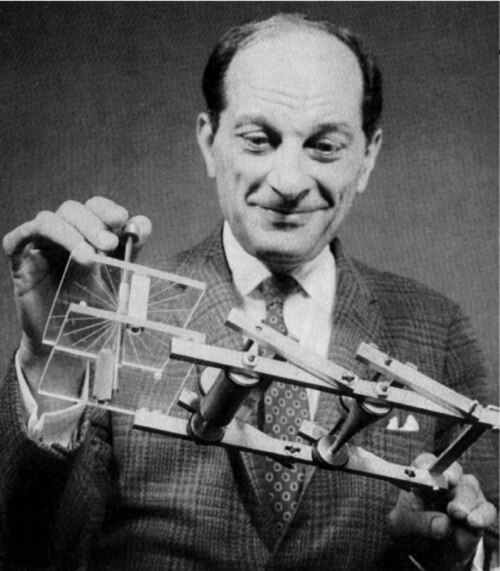
\includegraphics[width=\textwidth]{images/people/ulam.jpg}
        \caption{Stanisław Ulam e il FERMIAC.}
        \label{fig:ulam}
    \end{subfigure}
    \hfill
    \begin{subfigure}[b]{0.36\textwidth}
        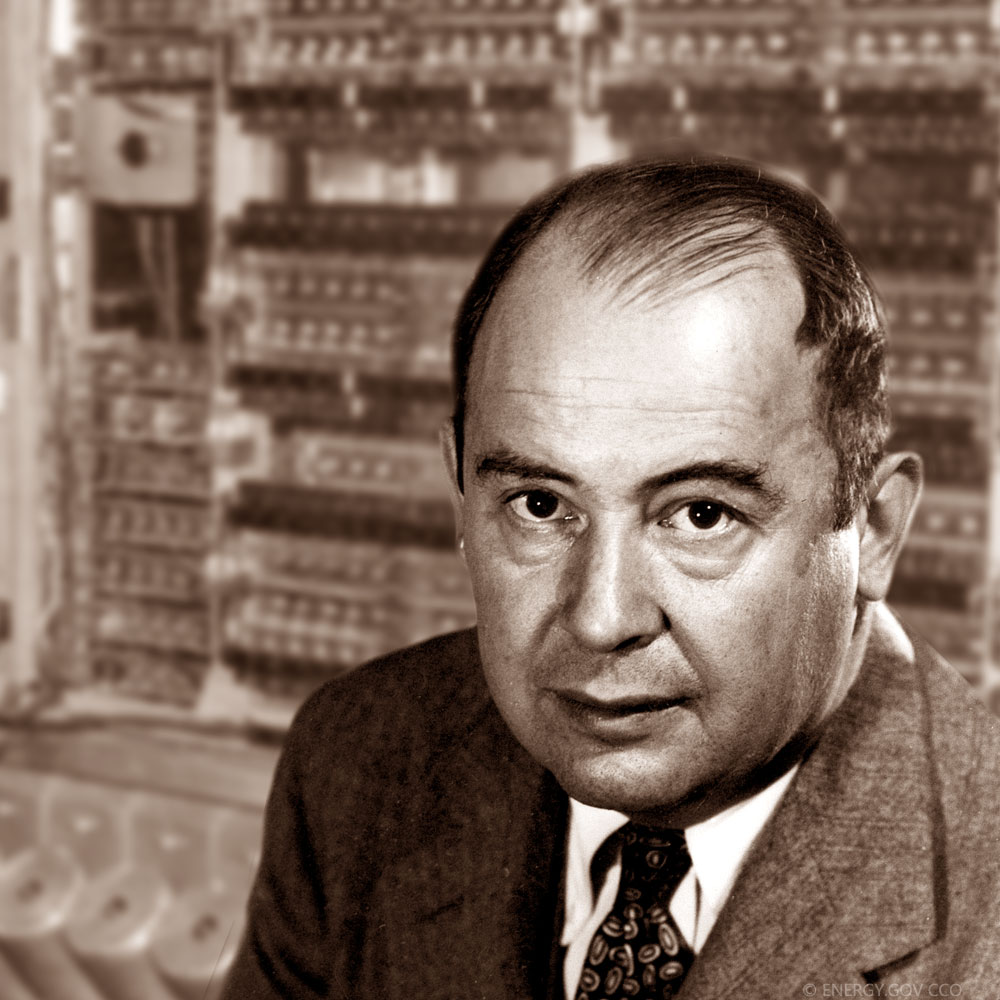
\includegraphics[width=\textwidth]{images/people/Von-Neumann-1000.jpg}
        \caption{Von Neumann.}
        \label{fig:von-neumann}
    \end{subfigure}
    \hfill
    \begin{subfigure}[b]{0.29\textwidth}
        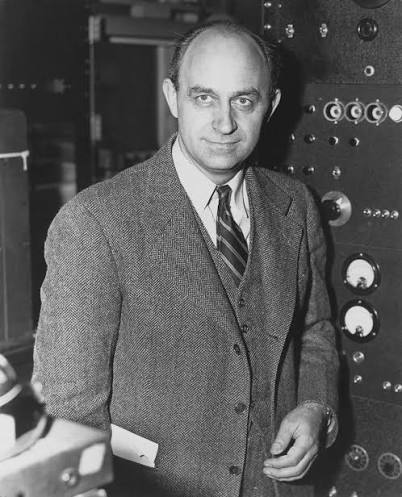
\includegraphics[width=\textwidth]{images/people/fermi.jpg}
        \caption{Enrico Fermi.}
        \label{fig:fermi}
    \end{subfigure}
    \caption{I pionieri del metodo Monte Carlo.}
    \label{fig:pionieri-mc}
\end{figure}

\section{Monte Carlo classico}
\label{sec:monte-carlo-classico}

\subsection{Metodo dell'inversa}
...

\section{Markov Chain Monte Carlo}
\label{sec:mcmc}
\subsection{Catene di Markov}

Sia ${X_1,..., X_N}$ una sequenza di variabili aleatorie in $\mathbb{R}^D$, questa sequenza è una catena di Markov se la probabilità condizionata di ogni $X_i$ soddisfa:

\begin{equation}
P(X_i |X_{i-1},..., X_{1}) = P(X_i | X_{i-1}).
\end{equation}

Dunque la probabilità di ottenere un certo valore di $X_i$ dipende solo dalla variabile aleatoria precedente della catena e non dalle altre, questa richiesta equivale a dire che la catena di Markov sono catene \textit{senza memoria}, ovvero che solo l'ultimo stato della catena influenza il prossimo stato \cite{quantum_monte_carlo_methods}. 
Considerando il caso che la variabile aleatoria $X_i$ possa assumere un numero discreto di valori, ovvero che $X_i \in \{x_1, ..., x_j, ...\}$, in questo modo possiamo descrivere la distribuzione di probabilità e le probabilità condizionate di tali variabili utilizzando un vettore e una matrice rispettivamente:
\begin{equation}
P(X_i) = p^{(i)}_j = \begin{pmatrix} p^{(i)}(x_1) \\ \vdots \\ p^{(i)}(x_j) \\ \vdots \end{pmatrix}, 
\quad
P(X_j|X_i) = P_{ij} = 
\begin{pmatrix}
P(x_1|x_1)  & \cdots & P(x_j|x_1) & \cdots \\
P(x_1|x_2) & \cdots & P(x_j|x_2) & \cdots \\
\vdots & \ddots & \vdots & \\
P(x_1|x_i) & \cdots & P(x_j|x_i) & \cdots \\
\vdots   & \vdots & \ddots
\end{pmatrix}
\end{equation}

Dove è possibile notare che le quantità $P_{ij}$, non dipendono dalle variabili nella sequenza che stiamo utilizzando grazie alle proprietà markoviane della catena. Inoltre possiamo notare alcune proprietà interessanti sia per $p^{(i)}_j$ che per $P_{ij}$, in quanto $\forall i$ esse soddisfano:
\begin{equation}
\sum_{j} p^{(i)}_j = 1, \quad \sum_{j} P_{ij} =1.
\label{ev_prob}
\end{equation}

Una catena di Markov è definita da una probabilità iniziale $p^{(0)}_i$ e da una matrice stocastica $P_{ij}$ detta \textbf{matrice di transizione}, poichè essa permette di generare la catena in modo ricorsivo:
\begin{equation}
    p^{(k+1)}_i = \sum_{j} P_{ij} p^{(k)}_j  \ \text{con } k \in \mathbb{N}.
\end{equation}

Questa evoluzione della distribuzione di probabilità della catena conserva la normalizzazione della distribuzione, infatti:
\begin{equation}
\sum_{i} p^{(k+1)}_i = \sum_{i} \sum_{j} P_{ij} p^{(k)}_j = \sum_{j} p^{(k)}_j \sum_{i} P_{ij} = \sum_{j} p^{(k)}_j = 1.
\end{equation}

Inoltre considerando una matrice di transizione ergodica(ovvero irriducibile e aperiodica) è assicurato che a prescindere dalla distribuzione iniziale $p^{(0)}_i$ iterando il procedimento si raggiunge una \textbf{distribuzione stazionaria} $p_i$ tale che:
\begin{equation}
    p_i = \sum_{j} P_{ij} p_j.
\end{equation}
Ovvero si raggiunge una distribuzione di probabilità che non viene più modificata iterando il procedimento (per questo detta stazionaria), inoltre essa è l'autovettore della matrice di transizione $P_{ij}$ con autovalore unitario.
L'obbiettivo di Markov Chain Monte Carlo è quello di costruire una catena di Markov che abbia come distribuzione stazionaria la distribuzione target $p_i$ che vogliamo campionare. Per fare ciò è necessario costruire una matrice di transizione $P_{ij}$ costruita in un certo modo. 

Metropolis et al. (1953) proposero che fosse possibile ottenere una specifica distribuzione $p_i$ se la $P_{ij}$ soddisfa una certa condizione di simmetria detta \textbf{bilancio dettagliato}: 
\begin{equation}
    P_{ij} p_j = P_{ji} p_i.
\end{equation}
Nella sezione successiva verrà presentato l'algoritmo di Metropolis, che permette di costruire una matrice di transizione $P_{ij}$ che soddisfa la condizione di bilancio dettagliato permettendo di campionare una distribuzione target $p_i$.

\subsection{Algoritmo di Metropolis}

Dunque per poter calcolare le quantità termodinamiche di interesse è necessaria una matrice di transizione che soddisfi il bilancio dettagliato per la distribuzione di Boltzmann.

Metropolis et al. proposero di costruire la matrice di transizione $P_{ij}$ come prodotto di due matrici:

\begin{equation}
P_{ij}=T_{ij}A_{ij},
\end{equation}
dove $T_{ij}$ è la matrice di proposta, che rappresenta la probabilità di proporre una transizione dallo stato $j$ allo stato $i$, e $A_{ij}$ è la matrice di accettazione, che rappresenta la probabilità di accettare la transizione proposta. Gli elementi della matrice di proposta $T_{ij}$ devono soddisfare le seguenti condizioni:
\begin{equation}
T_{ij} \ge 0, \quad \sum_{i} T_{ij} = 1 \quad \forall j, \quad T_{ij} = T_{ji}.
\end{equation}
Mentre gli elementi della matrice di accettazione $A_{ij}$ sono costruiti in modo che:
\begin{equation}
    A_{ij} = \min\left(1, \frac{p_i}{p_j}\right).
\end{equation}
Queste condizioni assicurando che la matrice di transizione rispetti il bilancio dettagliato, e quindi che la distribuzione stazionaria della catena di Markov sia la distribuzione target $p_i$, infatti (assumendo $p_i \le p_j$ senza perdita di generalità):
\begin{equation}
 P_{ij} = T_{ij}A_{ij} = T_{ji} \frac{p_i}{p_j} = P_{ji} \frac{p_i}{p_j} \implies P_{ij} p_j = P_{ji} p_i.
\end{equation}
L'algoritmo di Metropolis è quindi un metodo per costruire una catena di Markov che campiona una distribuzione target $p_i$ senza la necessità di conoscere la costante di normalizzazione della distribuzione, il seguente pseudocodice descrive l'operazione base dell'algoritmo di Metropolis:
\\
\newline
\begin{algorithm}[H]
\SetAlgoLined
\KwIn{Configurazione $X^{(i)}$; distribuzione target $p(x)$ nota a meno della costante di normalizzazione; distribuzione di proposta simmetrica $T$.}
    Genera uno stato proposto $X' \sim T(X^{(k)})$\;

    Calcola la probabilità di accettazione \ \ $ A=\min (1,\frac{p(X')}{p(X^{(k)})}); $

    Genera $u\sim\mathcal U(0,1)$\;

    \eIf{$u\le A$}{
        \Return $X'$\;
    }{
        \Return $X^{(i)}$\;
    }
\KwOut{Configurazione $X^{(i+1)}$.}
\caption{Operazione base dell'algoritmo di Metropolis}
\label{alg:metropolis}
\end{algorithm}
\vspace{5mm}
L'iterazione di questa operazione è l'algoritmo di Metropolis, che è possibile vedere rappresentato graficamente in figura \ref{fig:metropolis}, dove si osservano i passi del camminatore randomico, una distribuzione proposta (prior), una distribuzione target (posterior) e i campioni generati dal metodo.

\begin{figure}[H]
    \centering
    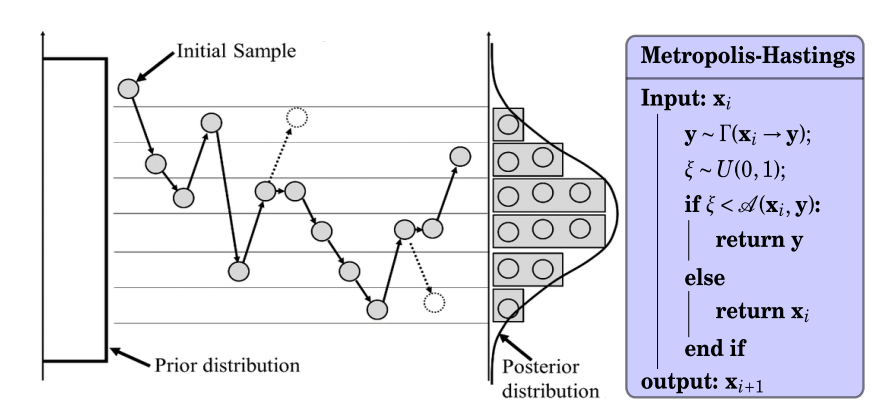
\includegraphics[width=0.9\textwidth]{images/MCMC/mcmc_algo.png}
    \caption{}
    \label{fig:metropolis}
\end{figure}

Dalla definizione della matrice di accettazione $A_{ij}$ è possibile notare che gli elementi di $P_{ij}$ dipendano esclusivamente dal rapporto della probabilità target nelle due configurzioni considerate (attuale e proposta), dunque sono indipendenti dalla costante di normalizzazione della distribuzione target. Come già espresso nel capitolo precedente, questo è un aspetto cruciale per il campionamento della distribuzione di Boltzmann, in quanto la costante di normalizzazione della distribuzione è proprio la funzione di partizione, di cui non è sempre possibile da calcolare analiticamente o numericamente.

Infine l'algoritmo di Metropolis trasferisce la responsabilità dell'ergodicità di $P_{ij}$ alla matrice $T_{ij}$. Se in un numero finito di passi $T_{ij}$ permette di raggiungere tutto lo spazio delle fasi, allora l'algoritmo di Metropolis è ergodico. Questo è un aspetto cruciale per il corretto funzionamento dell'algoritmo, in quanto la catena di Markov deve essere in grado di esplorare tutto lo spazio delle configurazioni per garantire che la distribuzione stazionaria sia effettivamente raggiunta. In altre parole, se la matrice di proposta $T_{ij}$ non consente di visitare tutte le configurazioni possibili, l'algoritmo potrebbe rimanere intrappolato in una regione dello spazio delle fasi, portando a stime errate delle quantità termodinamiche.
\section{Campioni autocorrelati}
\label{sec:campioni-autocorrelati}

\subsection{Blocking Analysis}

\subsection{Metodo di Sokal}
\chapter{Normalizing Flows}

\section{Cambio di variabili e funzioni invertibili}

\section{Normalizing Flows}

\subsection{Espressività del Flow}

\subsection{Campionamento, inferenza ed addestramento}

\subsection{Costruire un Flow tramite composizione finita}

\subsection{Coupling Flow}

\subsection{Trasformazione affine}

\subsection{Coupling layers}

\subsection{Real NVP}

\subsection{Esempi}

\section{Flow Markov Chain Monte Carlo}
\chapter{Studio del campionamento}
\label{ch:studio}

Nei capitoli precedenti sono stati introdotti gli strumenti teorici necessari a campionare una distribuzione di Boltzmann: il campionamento markoviano locale via Metropolis-Hastings (Sez.~\ref{sec:mcmc}), i normalizing flow (Capitolo~\ref{ch:nf}) e da quest'ultimo è stato derivato anche uno schema ibrido, il Flow-MCMC. Questi tre metodi condividono l'obiettivo ma differiscono radicalmente nella strategia: MCMC locale esplora lo spazio delle configurazioni muovendosi solo nell'intorno immediato dello stato corrente; il normalizing flow genera campioni indipendenti, pagando il prezzo di un addestramento preliminare e di un possibile disallineamento tra la distribuzione appresa e quella target; il Flow-MCMC combina le due prospettive mantenendo convergenza asintotica e campionamento globale. La domanda naturale è se questa differenza di strategia si traduca in una differenza pratica misurabile nella qualità del campionamento.

Per rispondere si è scelto, come sistema di test, un potenziale a doppio pozzo lungo una coordinata, descritto in Sezione~\ref{sec:potenziale_dw}. Questo sistema ha la minima richiesta di multimodalità, essendo bimodale, e dunque è il caso più semplice in cui ci si aspetta che le strategie locali di campionamento, come Metropolis-Hastings standard, entrino in difficoltà; alla coordinata bimodale si possono affiancare ulteriori dimensioni puramente armoniche, che non aggiungono multimodalità ma permettono di studiare l'effetto della dimensionalità complessiva del sistema sulla qualità del campionamento.

Lo studio si articola in due parti. Nella Sezione~\ref{sec:limiti_mcmc} si studia il comportamento termodinamico del sistema utilizzando solo MCMC locale al variare del numero di dimensioni del sistema, mantenendo sempre la prima variabile nel doppio pozzo e aggiungendo un numero crescente di dimensioni armoniche,quantificando il fallimento attraverso l'acceptance rate, il tempo di autocorrelazione integrato. La Sezione~\ref{sec:confronto_metodi} confronta invece i tre metodi --- MCMC locale, NF con re-weighting e Flow-MCMC --- a dimensione fissata $D=3$ (una variabile in potenziale doppio pozzo e due armoniche), sia al variare della temperatura sia al variare del numero di campioni utilizzati. 

\section{Il potenziale doppio pozzo}
\label{sec:potenziale_dw}

Il potenziale doppio pozzo è definito da
\begin{equation}
    V_{\text{dw}}(x) = \frac{a}{b^4}\left(x^2 - b\right)^2,
\end{equation}
e viene scelto agente lungo una sola coordinata, mentre le rimanenti $D-1$ direzioni sono trattate come oscillatori armonici disaccoppiati. Il potenziale totale, per $\mathbf{x} = (x_1, \mathbf{x}_\perp) \in
\mathbb{R}^D$, è quindi
\begin{equation}
    V(\mathbf{x}) = \underbrace{\frac{a}{b^4}\left(x_1^2 - b\right)^2}_{V_{\text{dw}}(x_1)}
    \;+\; \underbrace{\frac{1}{2}\sum_{i=2}^{D} x_i^2}_{V_{\text{arm}}(\mathbf{x}_\perp)},
    \qquad a, b > 0.
    \label{eq:double_well_potential}
\end{equation}
La coordinata $x_1$ è detta "lenta",poichè vede la struttura a doppia buca, mentre $\mathbf{x}_\perp = (x_2,\dots,x_D)$ raccoglie le direzioni "veloci", puramente armoniche e prive di barriere.
Il termine $V_{\text{dw}}(x_1)$ ha due minimi in $x_1 = \pm\sqrt{b}$, separati da una barriera in $x_1 = 0$ di altezza
%
\begin{equation}
    \Delta V = V_{\text{dw}}(0) = \frac{a}{b^2}.
    \label{eq:barrier_height}
\end{equation}
%
Il potenziale è pari su ogni variabile, $V(-x_i) = V(x_i)$, e la distribuzione di Boltzmann associata eredita la stessa simmetria, $p(-x_i) = p(x_i)$. Una conseguenza diretta è il segno medio $\langle \operatorname{sgn}(x_1) \rangle$ è nullo, infatti:
\begin{equation}
    \langle \operatorname{sgn}(x_1) \rangle
    = \int_{\mathbb{R}^D} p(\mathbf{x}) \, \operatorname{sgn}(x_1) \, d\mathbf{x}.
\end{equation}
Operando il cambio di variabile $x_1 \to -x_1$ (a $\mathbf{x}_\perp$ fissato,
con $d\mathbf{x}$ invariante) si ottiene
\begin{equation}
    \langle \operatorname{sgn}(x_1) \rangle
    = \int_{\mathbb{R}^D} p(-x_1, \mathbf{x}_\perp) \, \operatorname{sgn}(-x_1) \, d\mathbf{x}
    = -\int_{\mathbb{R}^D} p(x_1, \mathbf{x}_\perp) \, \operatorname{sgn}(x_1) \, d\mathbf{x}
\end{equation}
dove nel secondo passaggio si è usata la parità di $p$ e la disparità di $\operatorname{sgn}$, $\operatorname{sgn}(-x_1) = -\operatorname{sgn}(x_1)$. Nell'ultimo passaggio possiamo risostituire la definizione di segno medio e da $\langle \operatorname{sgn}(x_1) \rangle = -\langle \operatorname{sgn}(x_1) \rangle$ segue immediatamente
\begin{equation}
    \langle \operatorname{sgn}(x_1) \rangle = 0.
\end{equation}

Nella simulazione si è fissato $a = 0.1$~eV e $b = 1.0$ (in unità della coordinata $x_1$), da cui, per l'Eq.~\eqref{eq:barrier_height}, una barriera $\Delta V = 0.1$~eV, con minimi in $x_1 = \pm 1$.

Il parametro rilevante per il grado di difficoltà del campionamento è il rapporto adimensionale $\Delta V / (k_B T)$ tra l'altezza della barriera e l'energia termica disponibile. Le temperature esplorate sono all'interno dell'intervallo $T \in [100, 1100]$~K e dunque il rapporto avrà un valore minimo e un valore massimo:
%
\begin{equation}
    \frac{\Delta V}{k_B T}\bigg|_{T = 1100~\text{K}} \approx 1.05,
    \qquad
    \frac{\Delta V}{k_B T}\bigg|_{T = 100~\text{K}} \approx 11.6.
\end{equation}
%
Alle temperature più alte la barriera è dell'ordine dell'energia termica: la catena di Markov con proposte locali la attraversa facilmente. Alle temperature più basse la barriera diventa fortemente soppressa in probabilità ($e^{-\Delta V/k_BT} \sim e^{-11.6} \approx 9\times10^{-6}$), è in questo regime che ci si aspetta il fallimento del campionamento locale, e il vantaggio dei metodi basati su normalizing flow.

Il termine armonico $V_{\text{arm}}(\mathbf{x}_\perp)$ è disaccoppiato da $x_1$ e, per equipartizione, contribuisce esattamente $\tfrac{1}{2}(D-1)k_BT$ all'energia media: la sua funzione è puramente quella di aggiungere gradi di libertà al sistema senza aggiungere barriere energetiche e quindi senza aggiungere altre variabili multimodali. Questa separabilità rende inoltre disponibile un riferimento per l'energia media, ottenuto per quadratura numerica 1D sulla sola coordinata $x_1$ e sommando il
contributo armonico in forma chiusa; questo valore $\langle E \rangle_{\text{esatto}}(T)$ verrà usato come riferimento nei confronti al variare di $N$ in Sezione~\ref{sec:confronto_metodi}. 

\section{Limiti di Markov Chain Monte Carlo}
\label{sec:limiti_mcmc}
\subsection{Dettagli implementativi}
\begin{figure}[H]
    \centering
    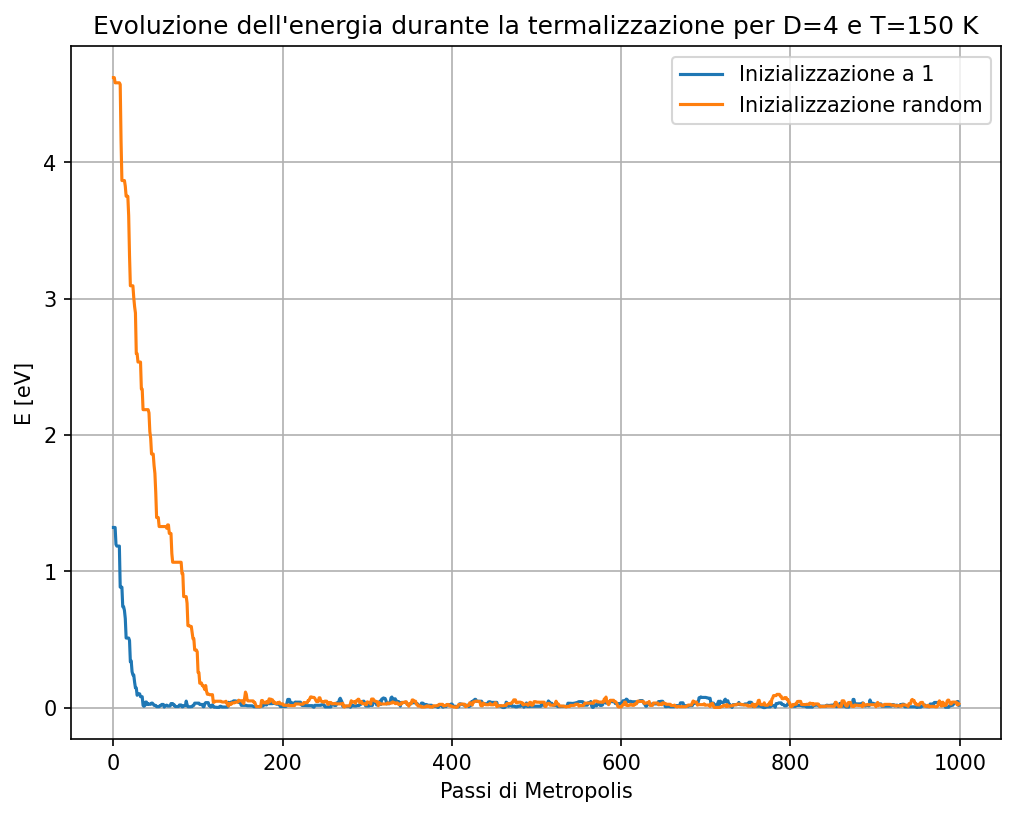
\includegraphics[width=0.9\textwidth]{images/MCMC/thermalization_energies_D4_T150.00.png}
    \caption{}
    \label{fig:therm_T_D}
\end{figure}

\subsection{Risultati}

\begin{figure}[H]
    \centering
    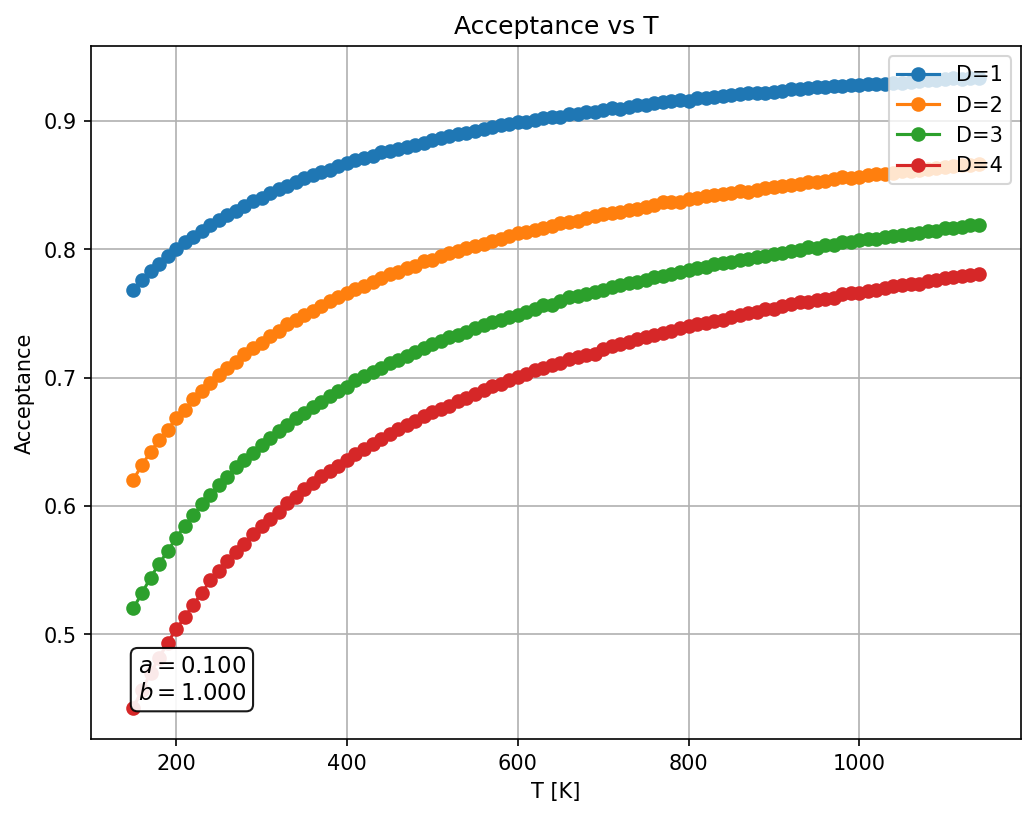
\includegraphics[width=0.9\textwidth]{images/MCMC/acceptance_vs_T.png}
    \caption{}
    \label{fig:acc_T_D}
\end{figure}

\begin{figure}[H]
    \centering
    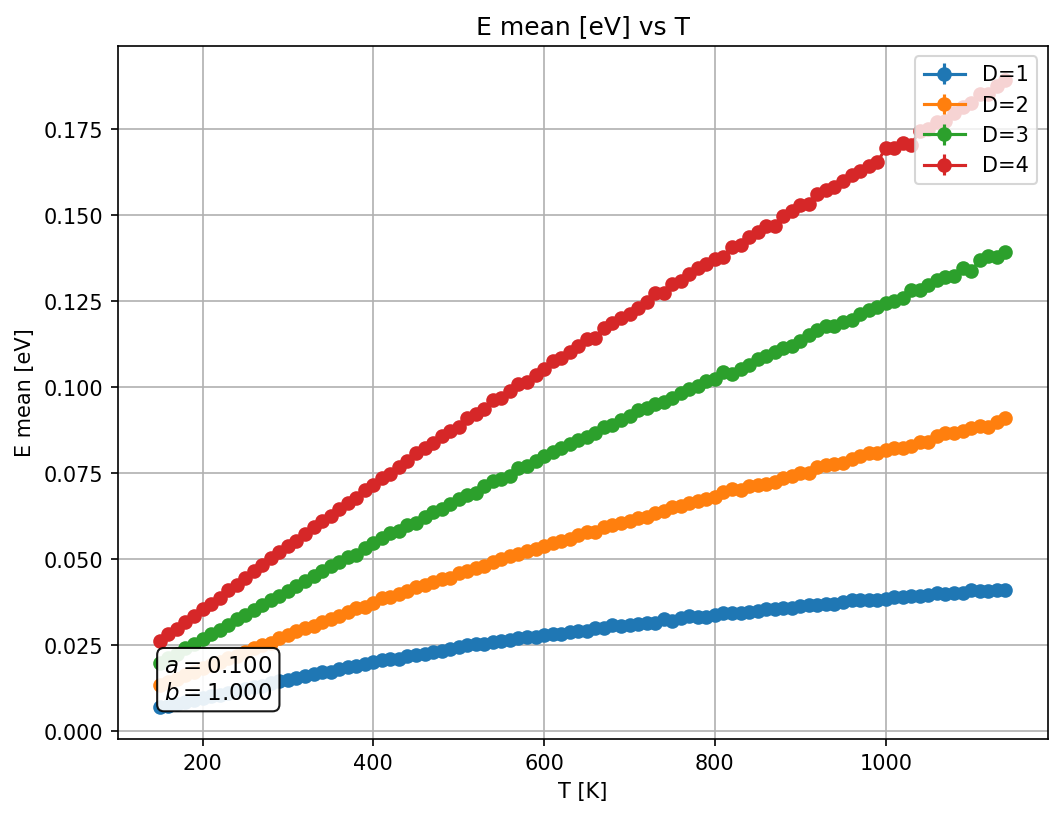
\includegraphics[width=0.9\textwidth]{images/MCMC/E_mean_vs_T.png}
    \caption{}
    \label{fig:E_T_D}
\end{figure}

\begin{figure}[H]
    \centering
    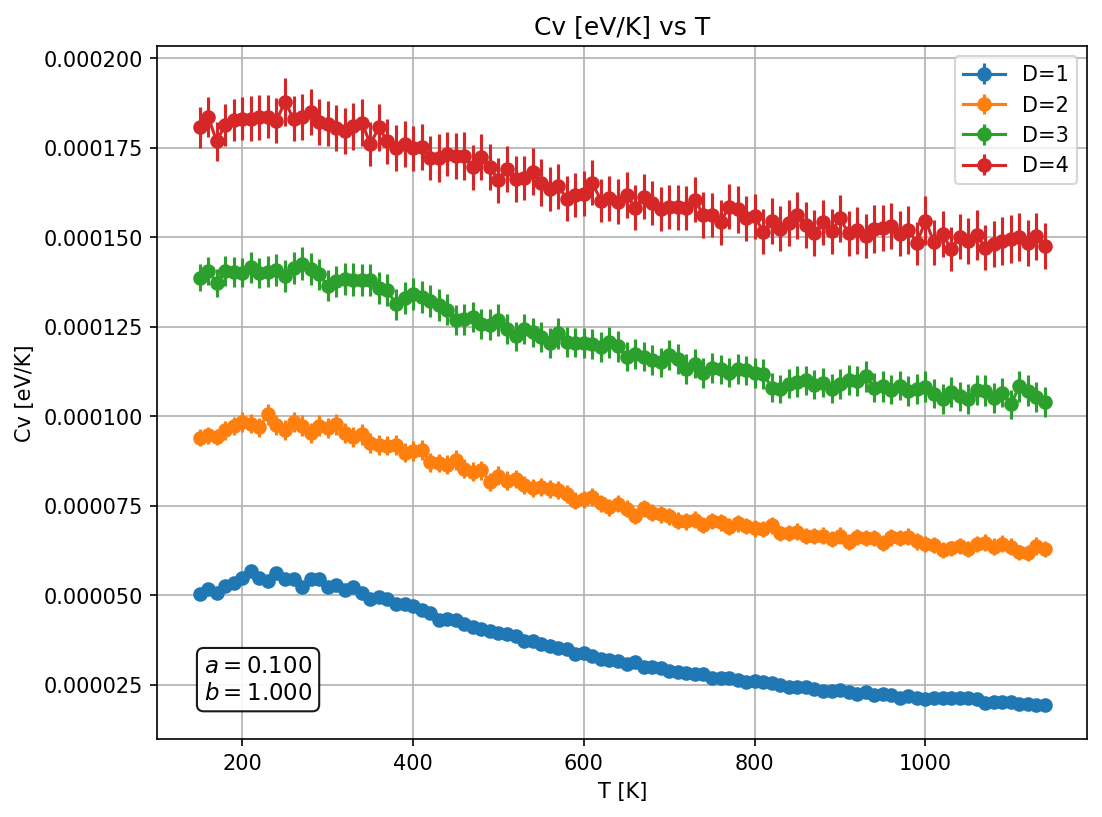
\includegraphics[width=0.9\textwidth]{images/MCMC/Cv_vs_T.png}
    \caption{}
    \label{fig:Cv_T_D}
\end{figure}

\begin{figure}[H]
    \centering
    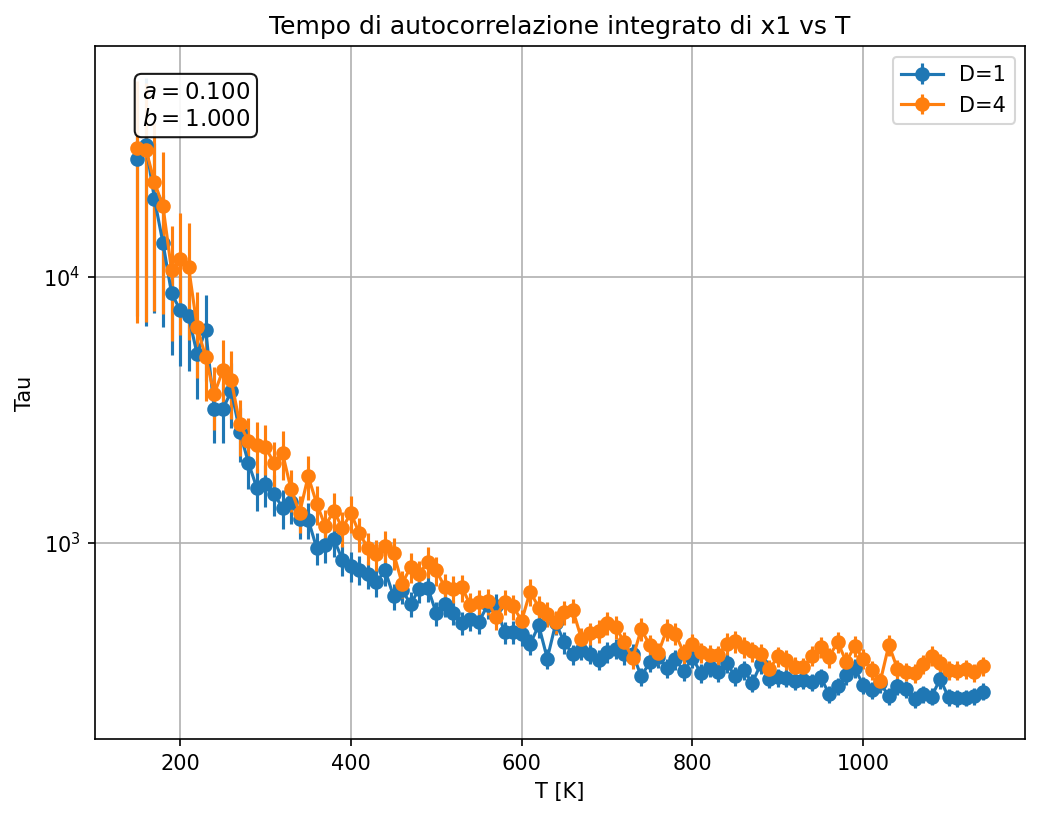
\includegraphics[width=0.9\textwidth]{images/MCMC/Tau_vs_T.png}
    \caption{}
    \label{fig:tau_T_D}
\end{figure}

\section{Confronto dei metodi di campionamento}
\label{sec:confronto_metodi}

\subsection{Dettagli implementativi}

\subsection{Confronto al variare di T}

\begin{figure}[H]
    \centering
    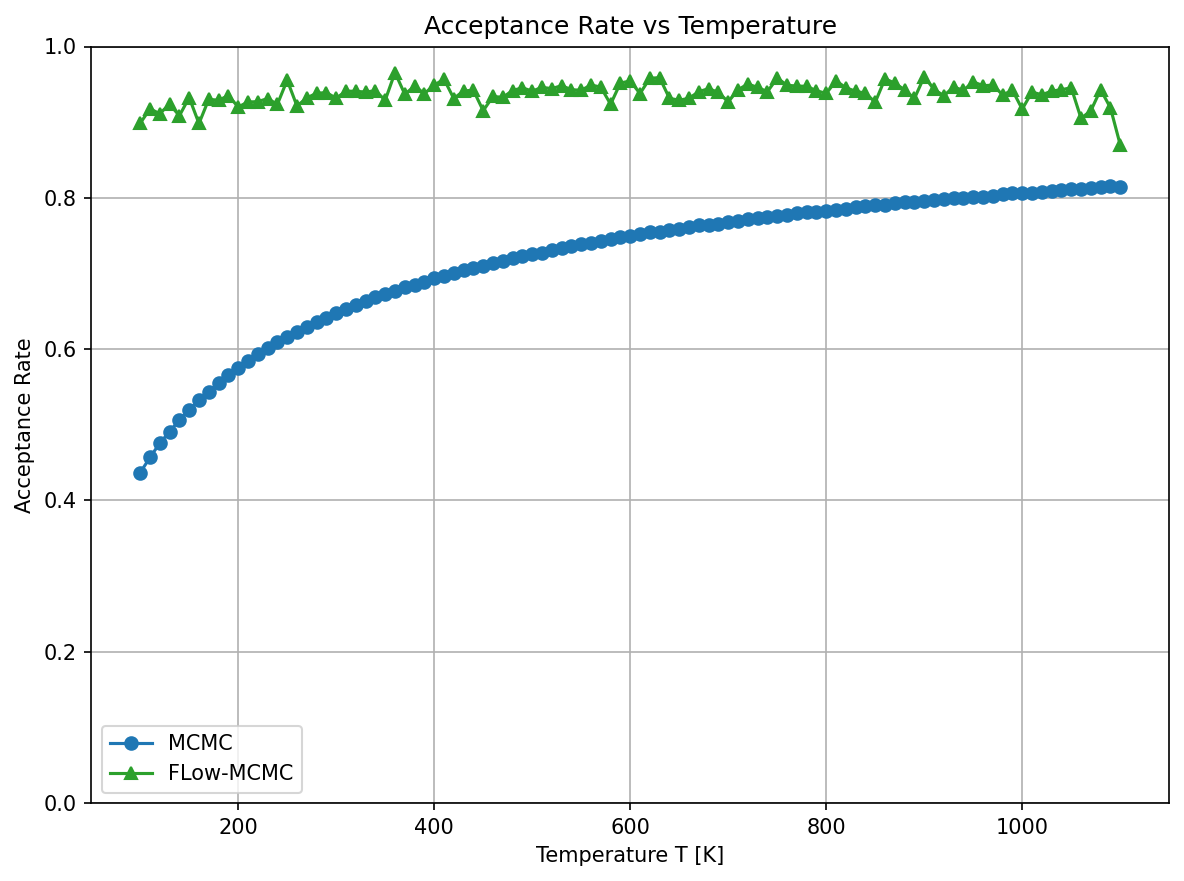
\includegraphics[width=0.9\textwidth]{images/acceptance_vs_T_plot.png}
    \caption{}
    \label{fig:acc_T_all}
\end{figure}

\begin{figure}[H]
    \centering
    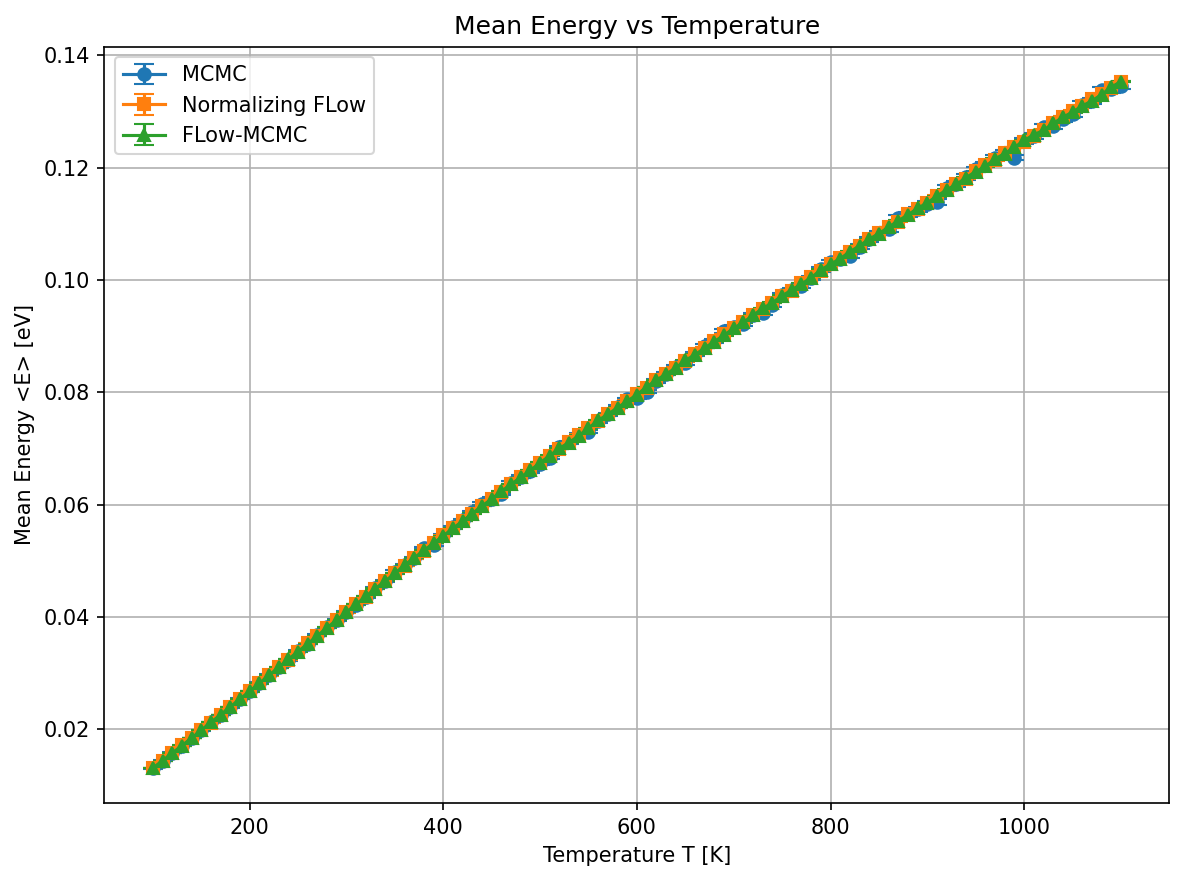
\includegraphics[width=0.9\textwidth]{images/E_vs_T_plot.png}
    \caption{}
    \label{fig:E_T_all}
\end{figure}

\begin{figure}[H]
    \centering
    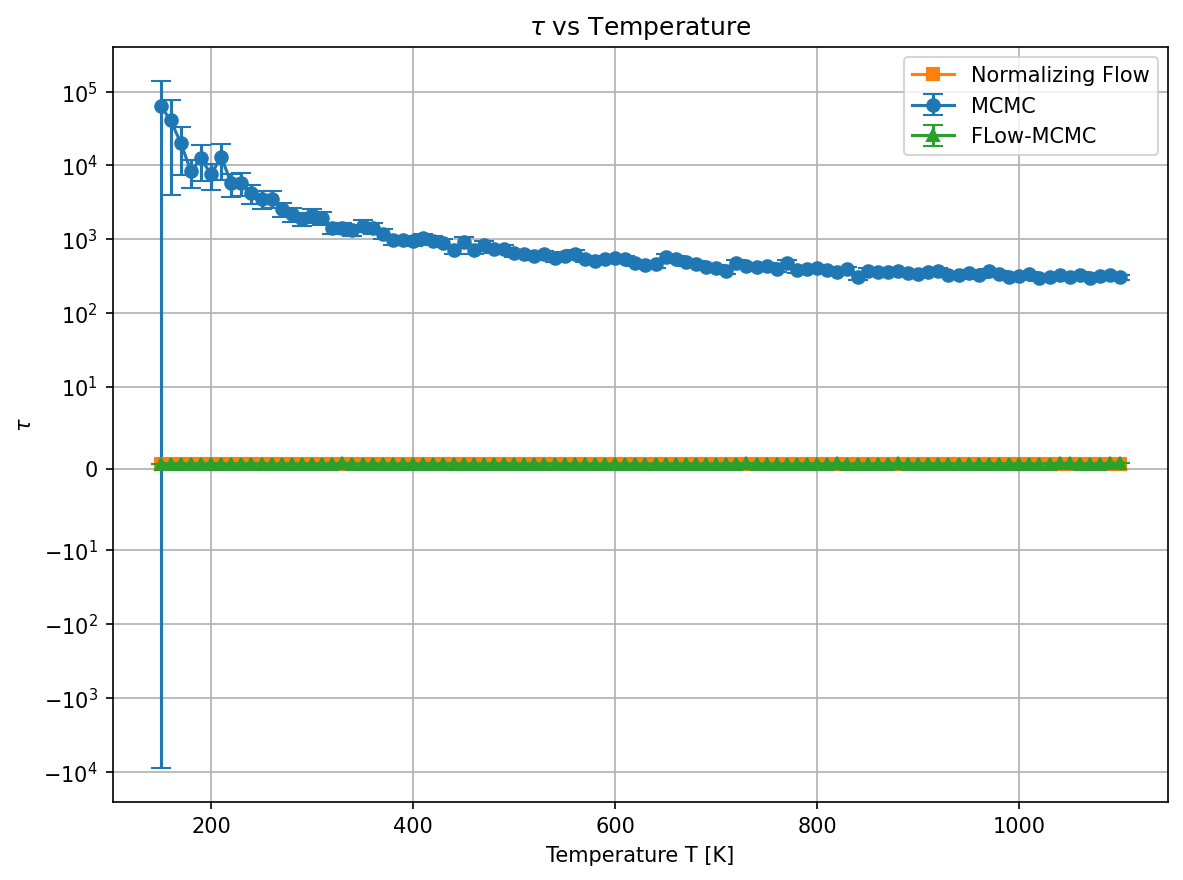
\includegraphics[width=0.9\textwidth]{images/tau_vs_T_plot.png}
    \caption{}
    \label{fig:tau_T_all}
\end{figure}

\begin{figure}[H]
    \centering
    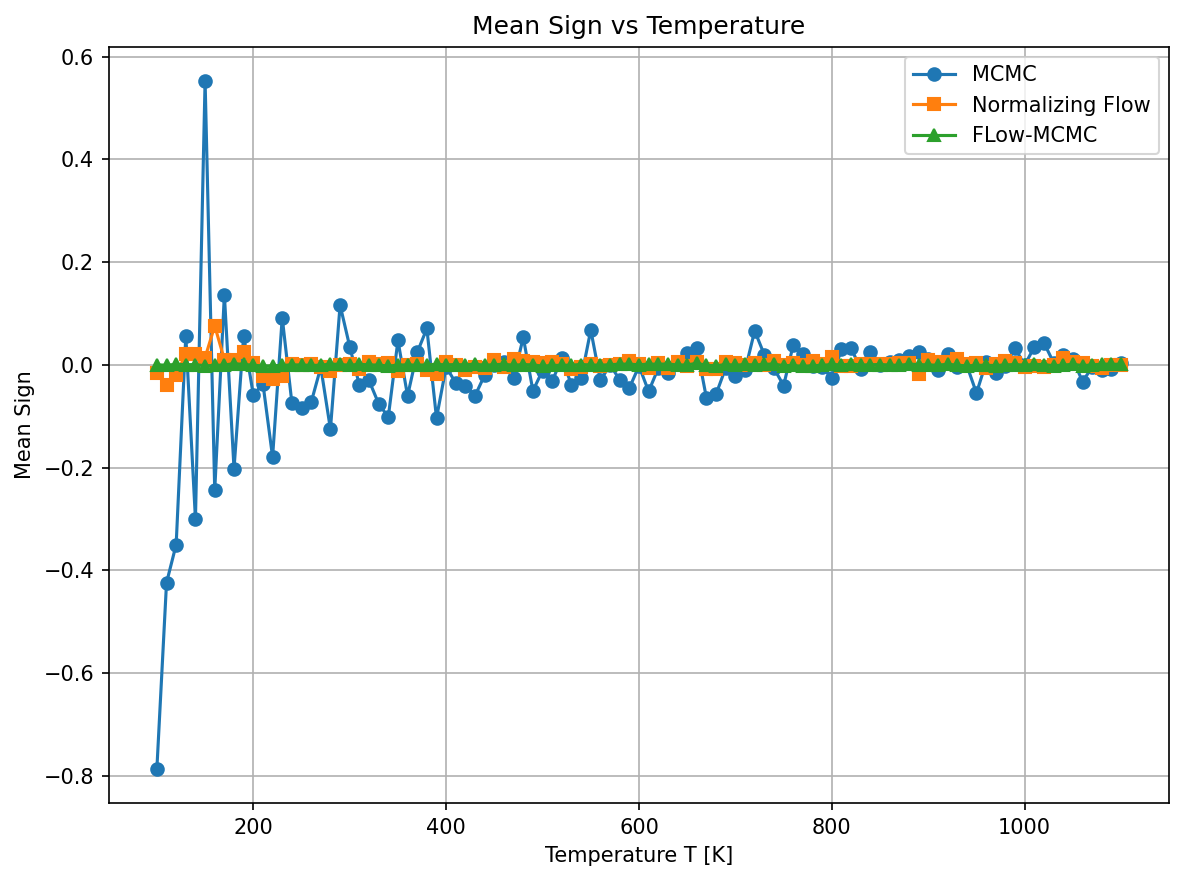
\includegraphics[width=0.9\textwidth]{images/mean_sign_vs_T_plot.png}
    \caption{}
    \label{fig:msig_T_all}
\end{figure}

\subsection{Confronto al variare di N}

\begin{figure}[H]
    \centering
    \begin{subfigure}[b]{0.45\textwidth}
        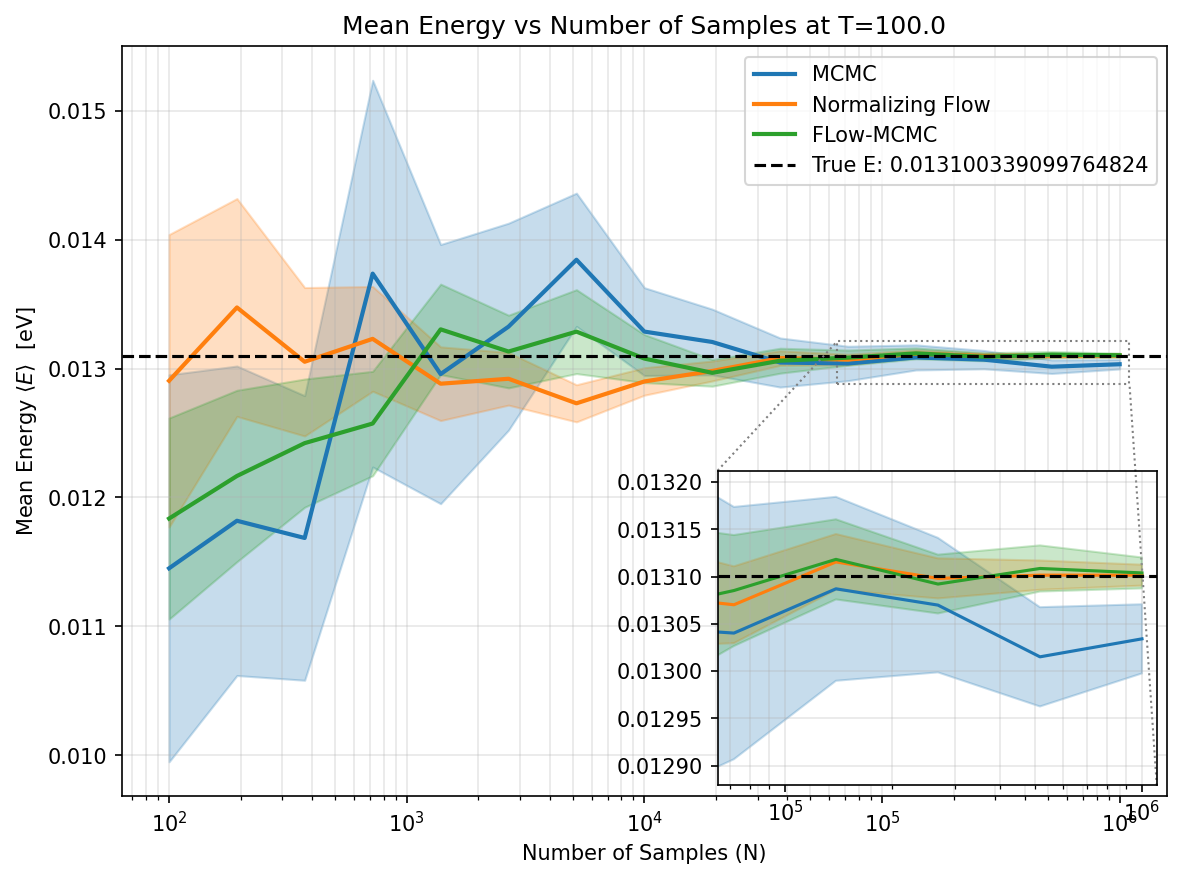
\includegraphics[width=\textwidth]{images/E_vs_N_plot_T_100.0.png}
        \caption{Prima}
    \end{subfigure}
    \hfill
    \begin{subfigure}[b]{0.45\textwidth}
        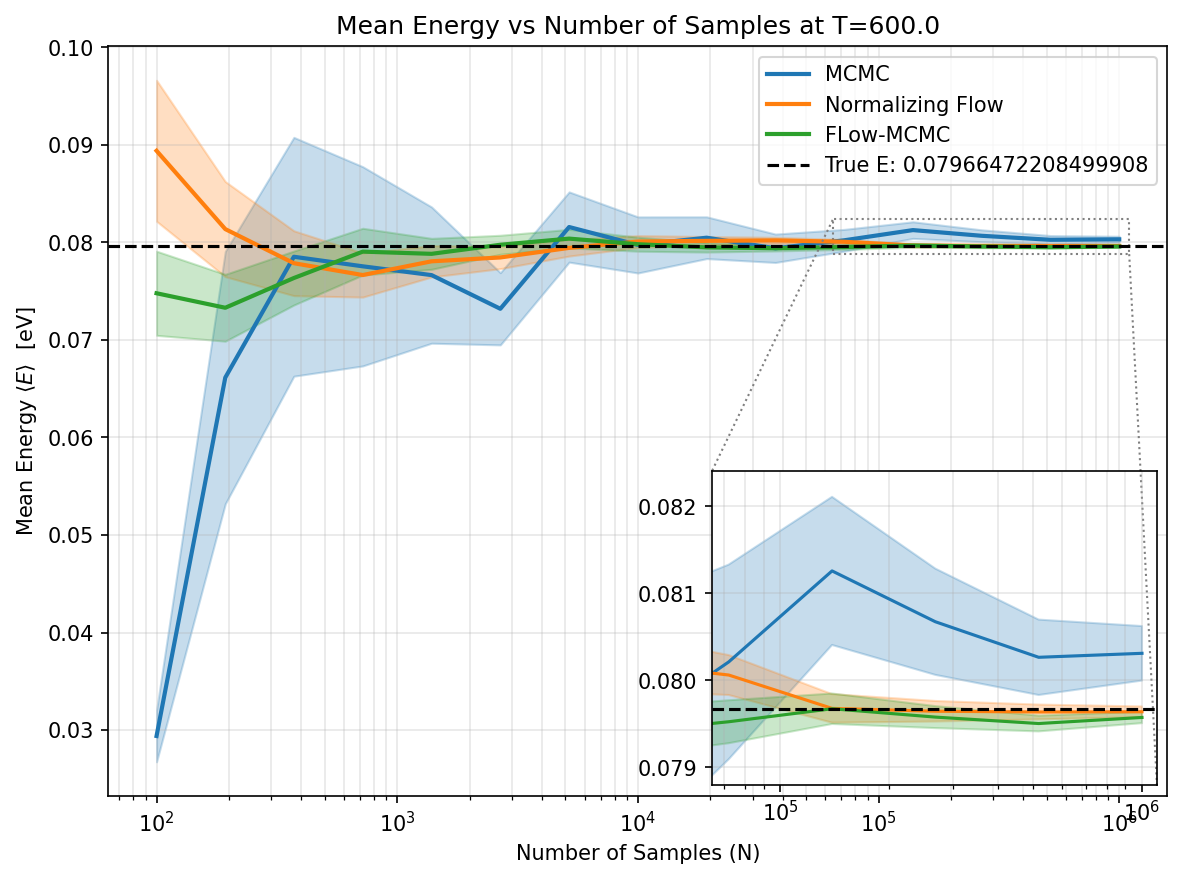
\includegraphics[width=\textwidth]{images/E_vs_N_plot_T_600.0.png}
        \caption{Seconda}
    \end{subfigure}
    
    \vspace{1em}
    
    \begin{subfigure}[b]{0.45\textwidth}
        \centering
        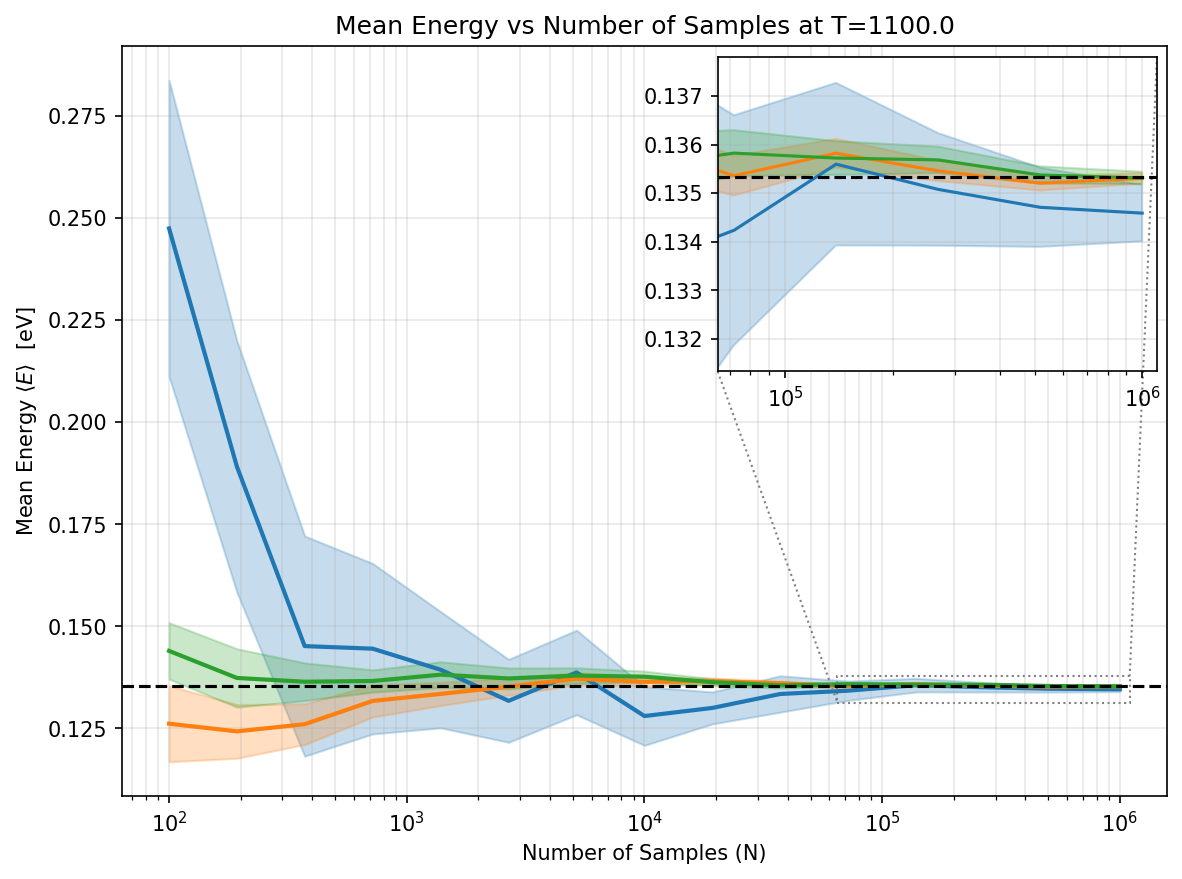
\includegraphics[width=\textwidth]{images/E_vs_N_plot_T_1100.0.png}
        \caption{Terza}
    \end{subfigure}
    \caption{}
\end{figure}

\begin{figure}[H]
    \centering
    \begin{subfigure}[b]{0.45\textwidth}
        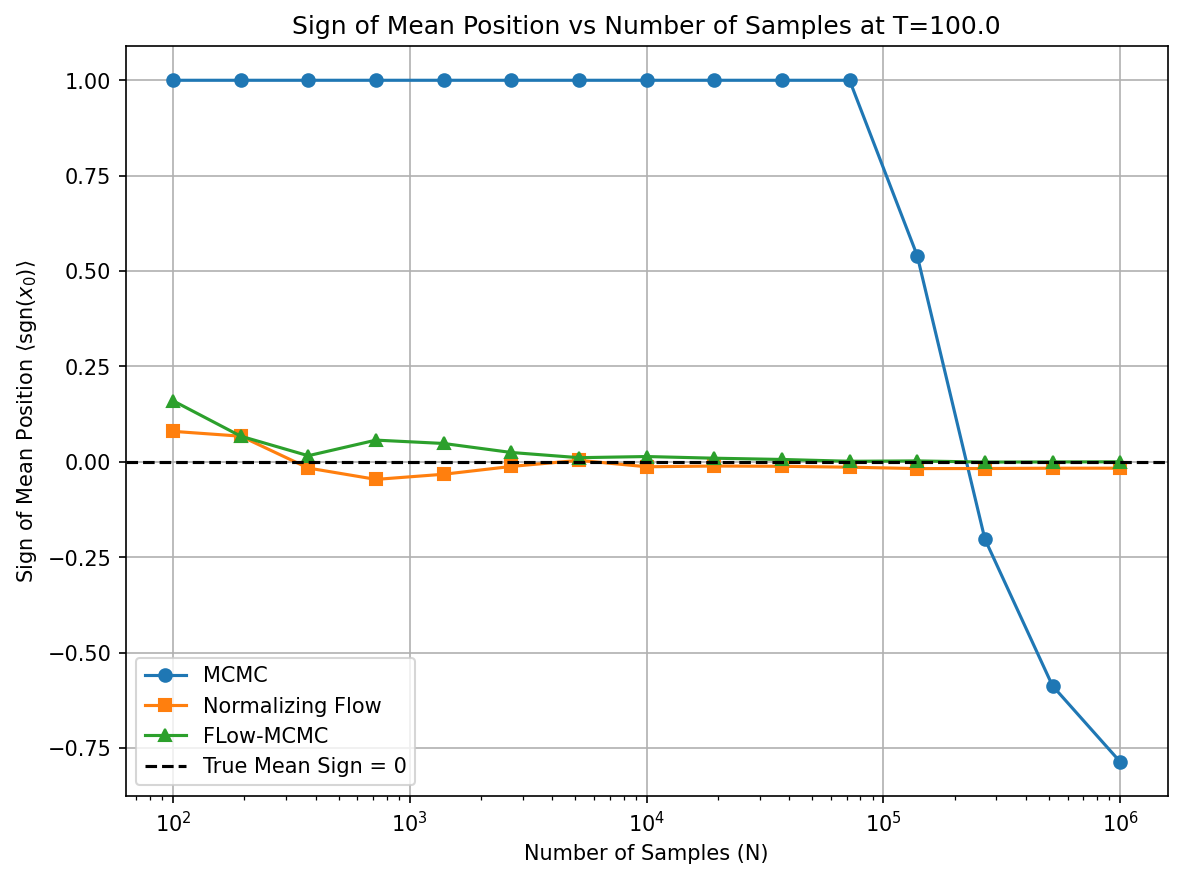
\includegraphics[width=\textwidth]{images/mean_sign_vs_N_plot_T_100.0.png}
        \caption{Prima}
    \end{subfigure}
    \hfill
    \begin{subfigure}[b]{0.45\textwidth}
        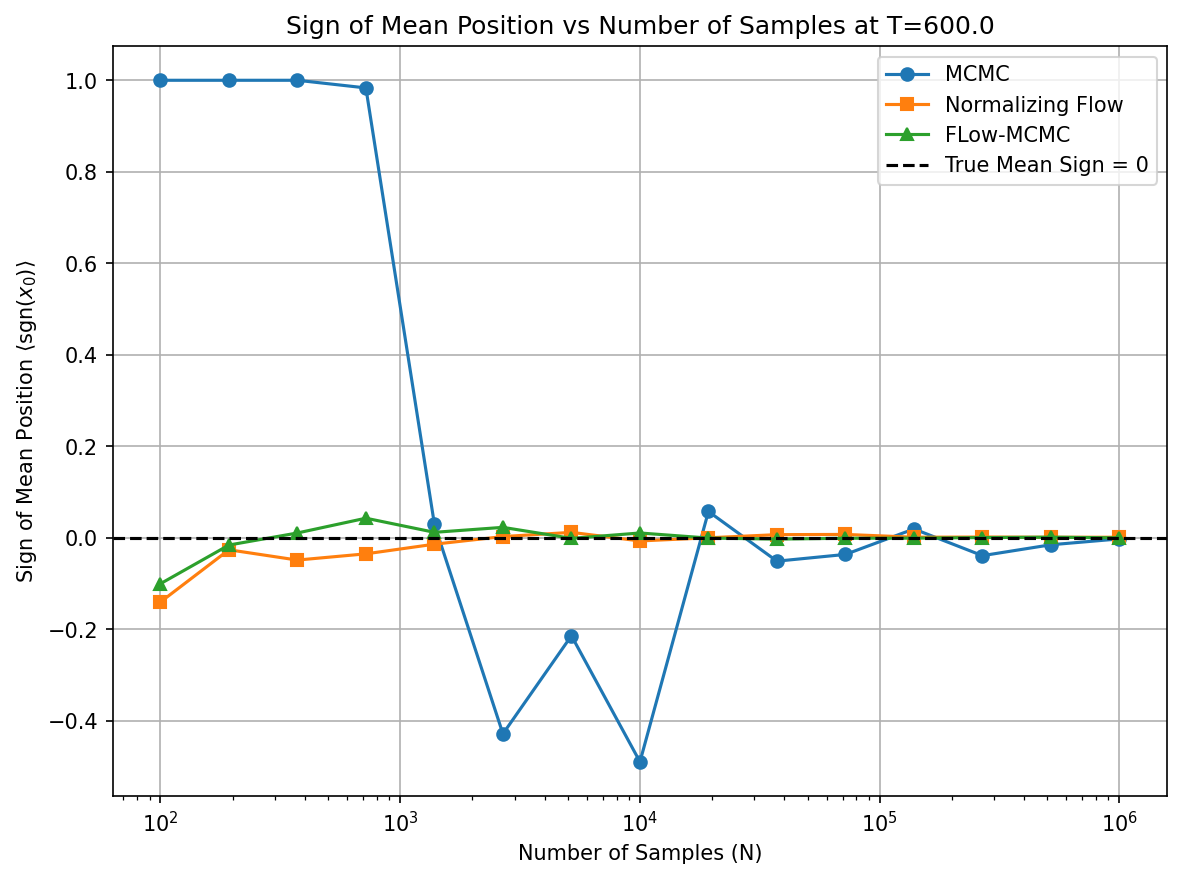
\includegraphics[width=\textwidth]{images/mean_sign_vs_N_plot_T_600.0.png}
        \caption{Seconda}
    \end{subfigure}
    
    \vspace{1em}
    
    \begin{subfigure}[b]{0.45\textwidth}
        \centering
        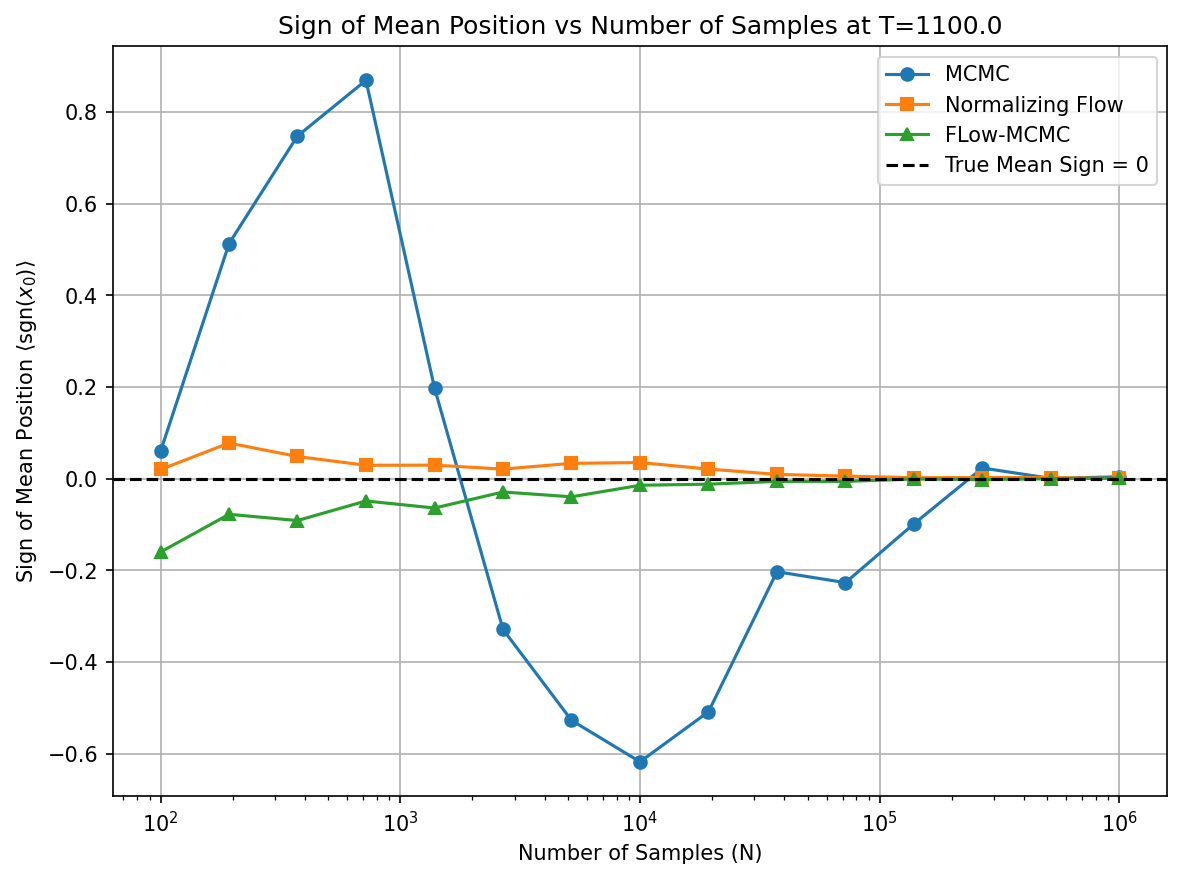
\includegraphics[width=\textwidth]{images/mean_sign_vs_N_plot_T_1100.0.png}
        \caption{Terza}
    \end{subfigure}
    \caption{}
\end{figure}

\subsection{Distribuzioni e traiettorie del camminatore}

\begin{figure}[H]
    \centering
    \begin{subfigure}[b]{0.45\textwidth}
        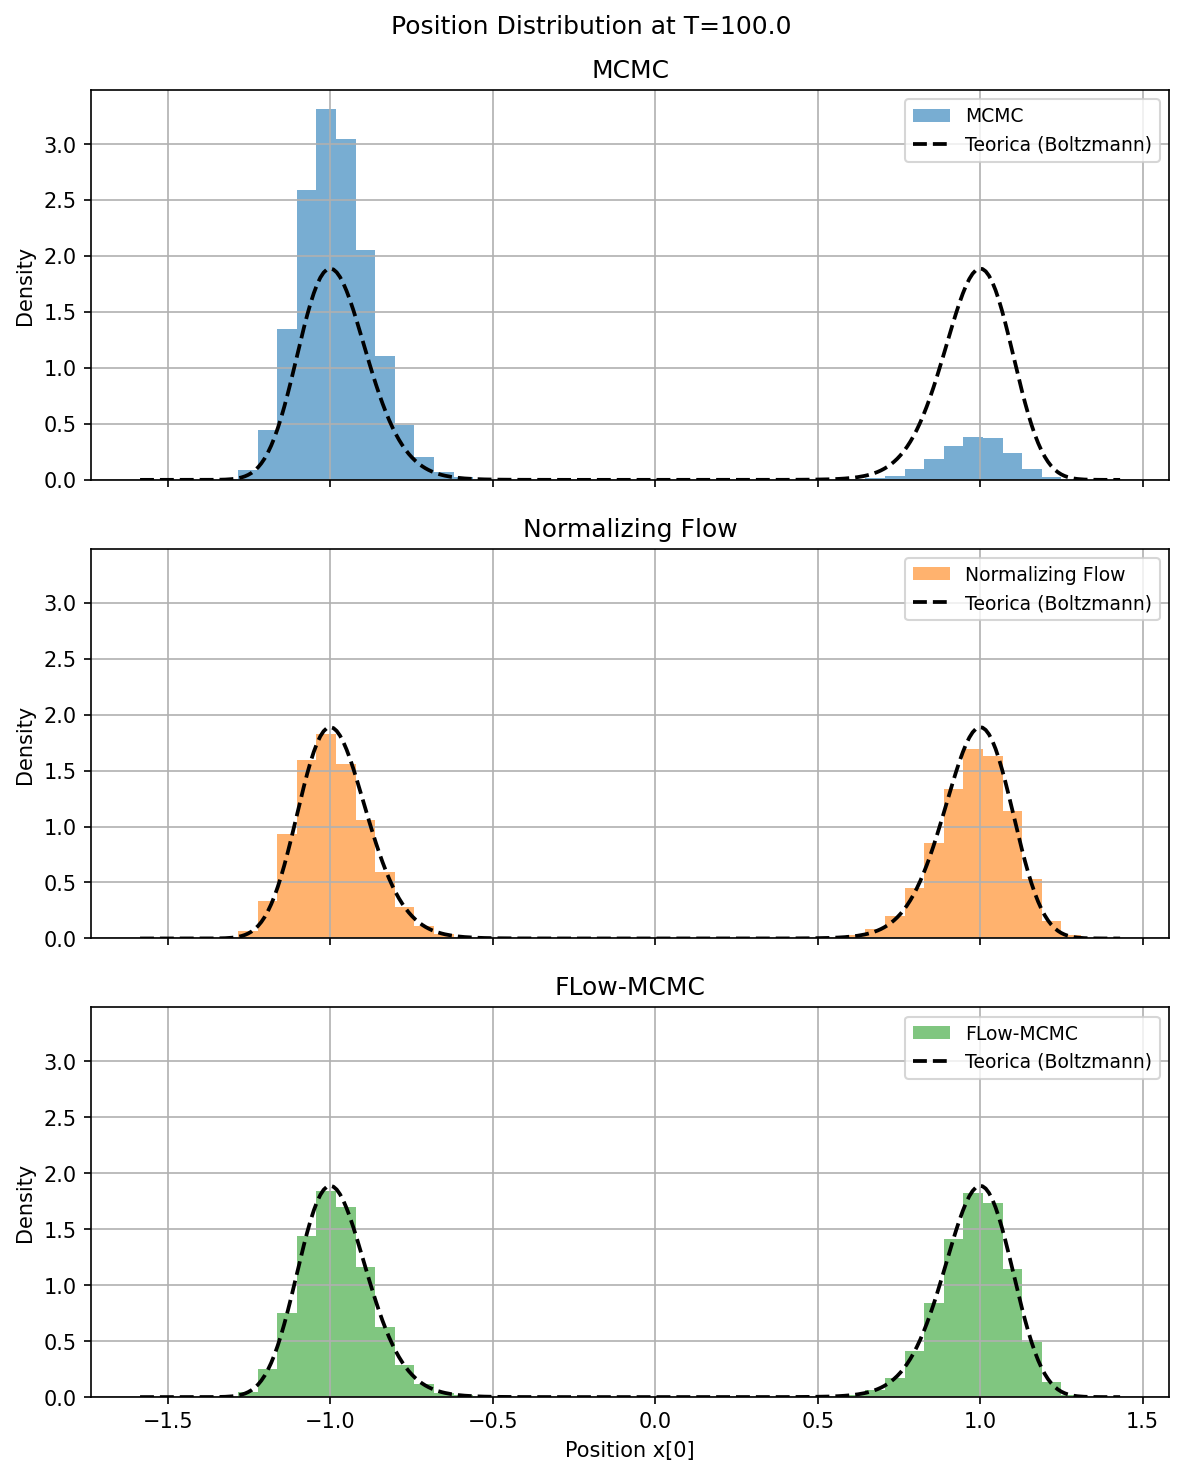
\includegraphics[width=\textwidth]{images/x_distribution_T_100.0.png}
        \caption{Prima}
    \end{subfigure}
    \hfill
    \begin{subfigure}[b]{0.45\textwidth}
        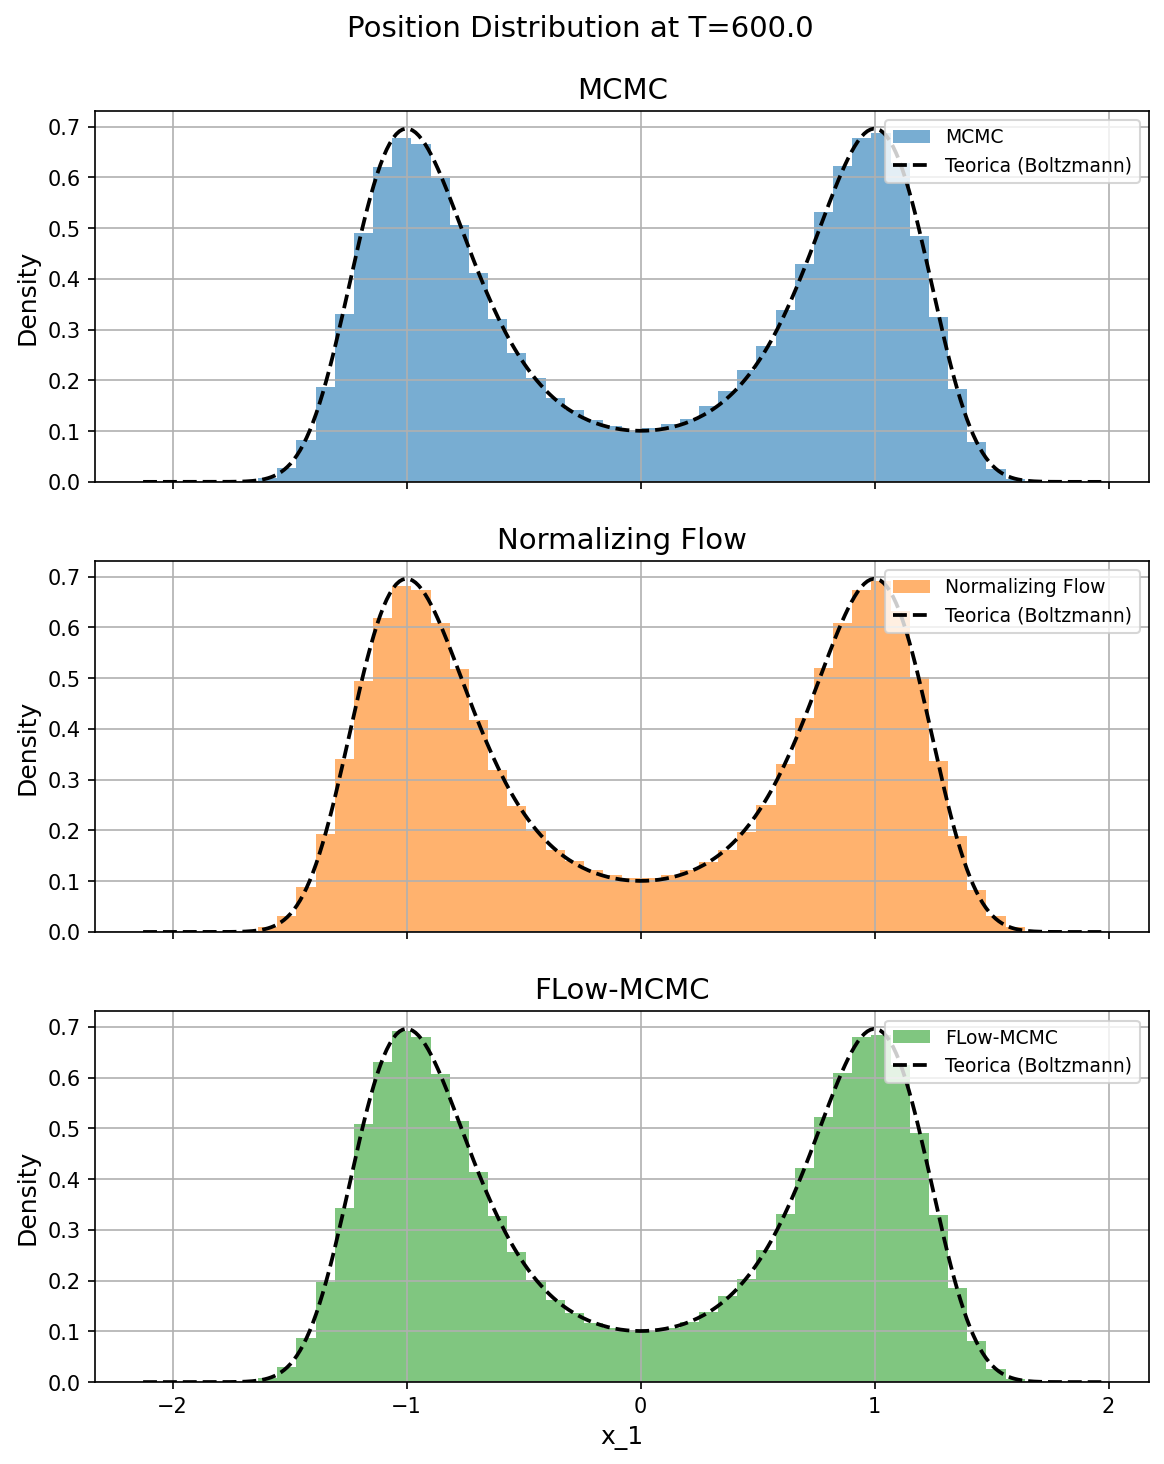
\includegraphics[width=\textwidth]{images/x_distribution_T_600.0.png}
        \caption{Seconda}
    \end{subfigure}
    
    \vspace{1em}
    
    \begin{subfigure}[b]{0.45\textwidth}
        \centering
        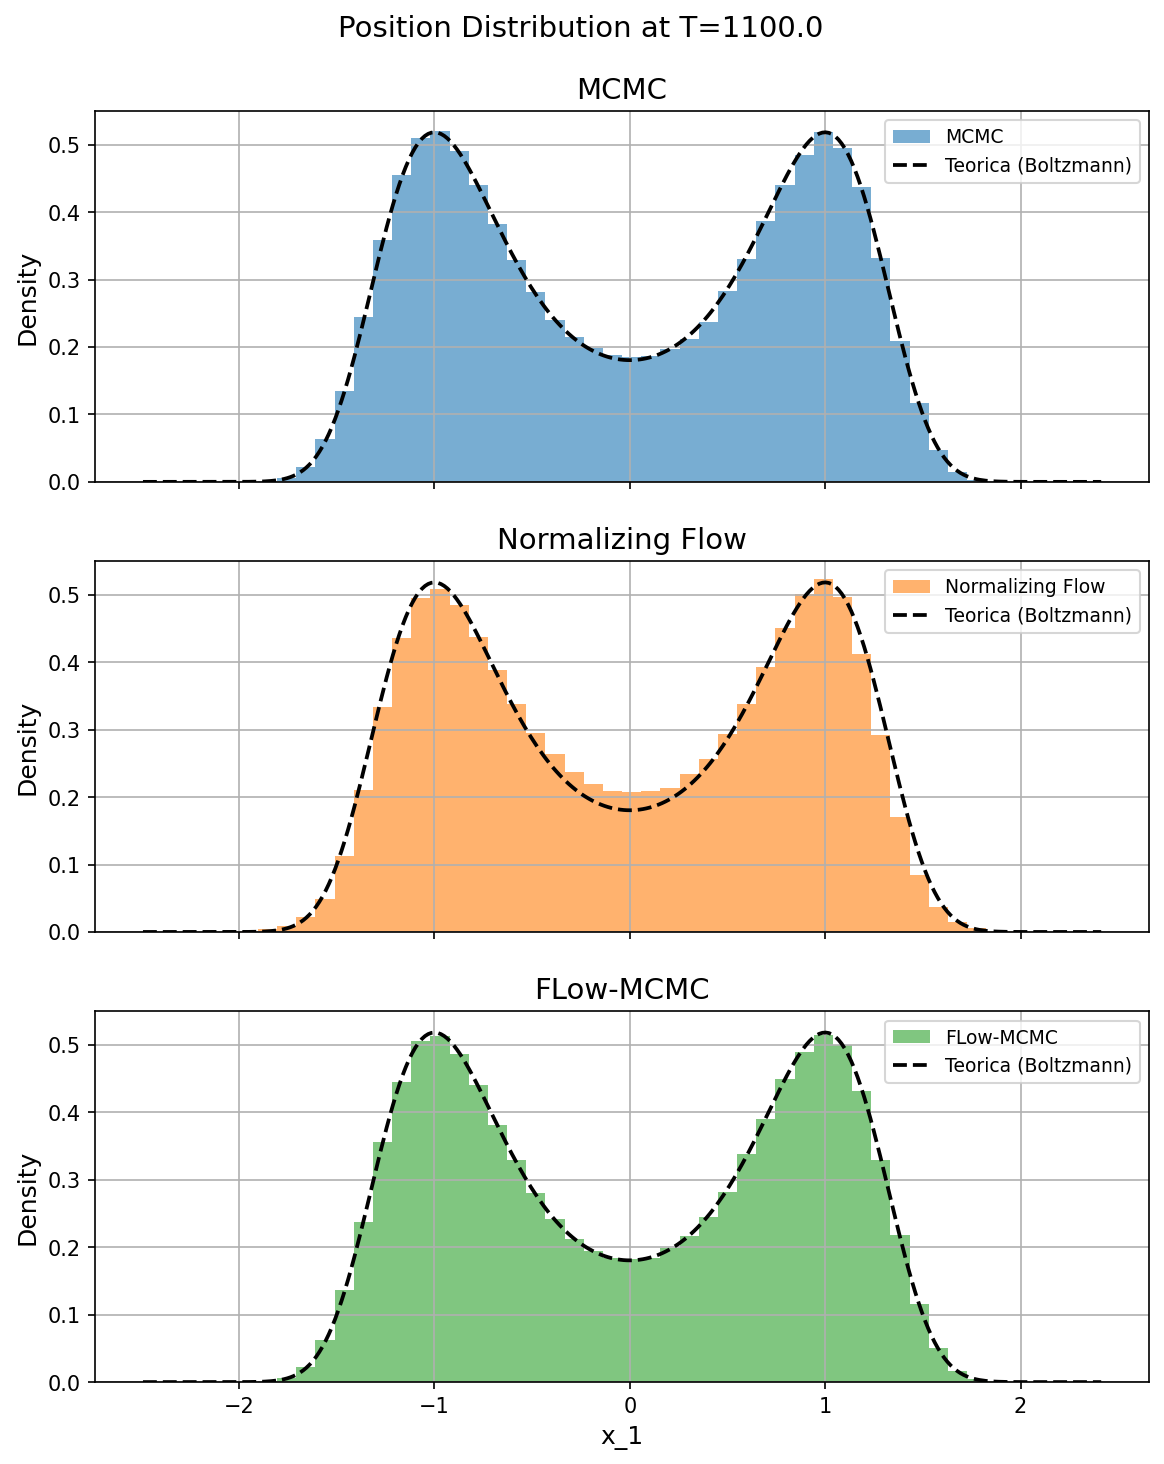
\includegraphics[width=\textwidth]{images/x_distribution_T_1100.0.png}
        \caption{Terza}
    \end{subfigure}
    \caption{}
\end{figure}

\begin{figure}[H]
    \centering
    \begin{subfigure}[b]{0.45\textwidth}
        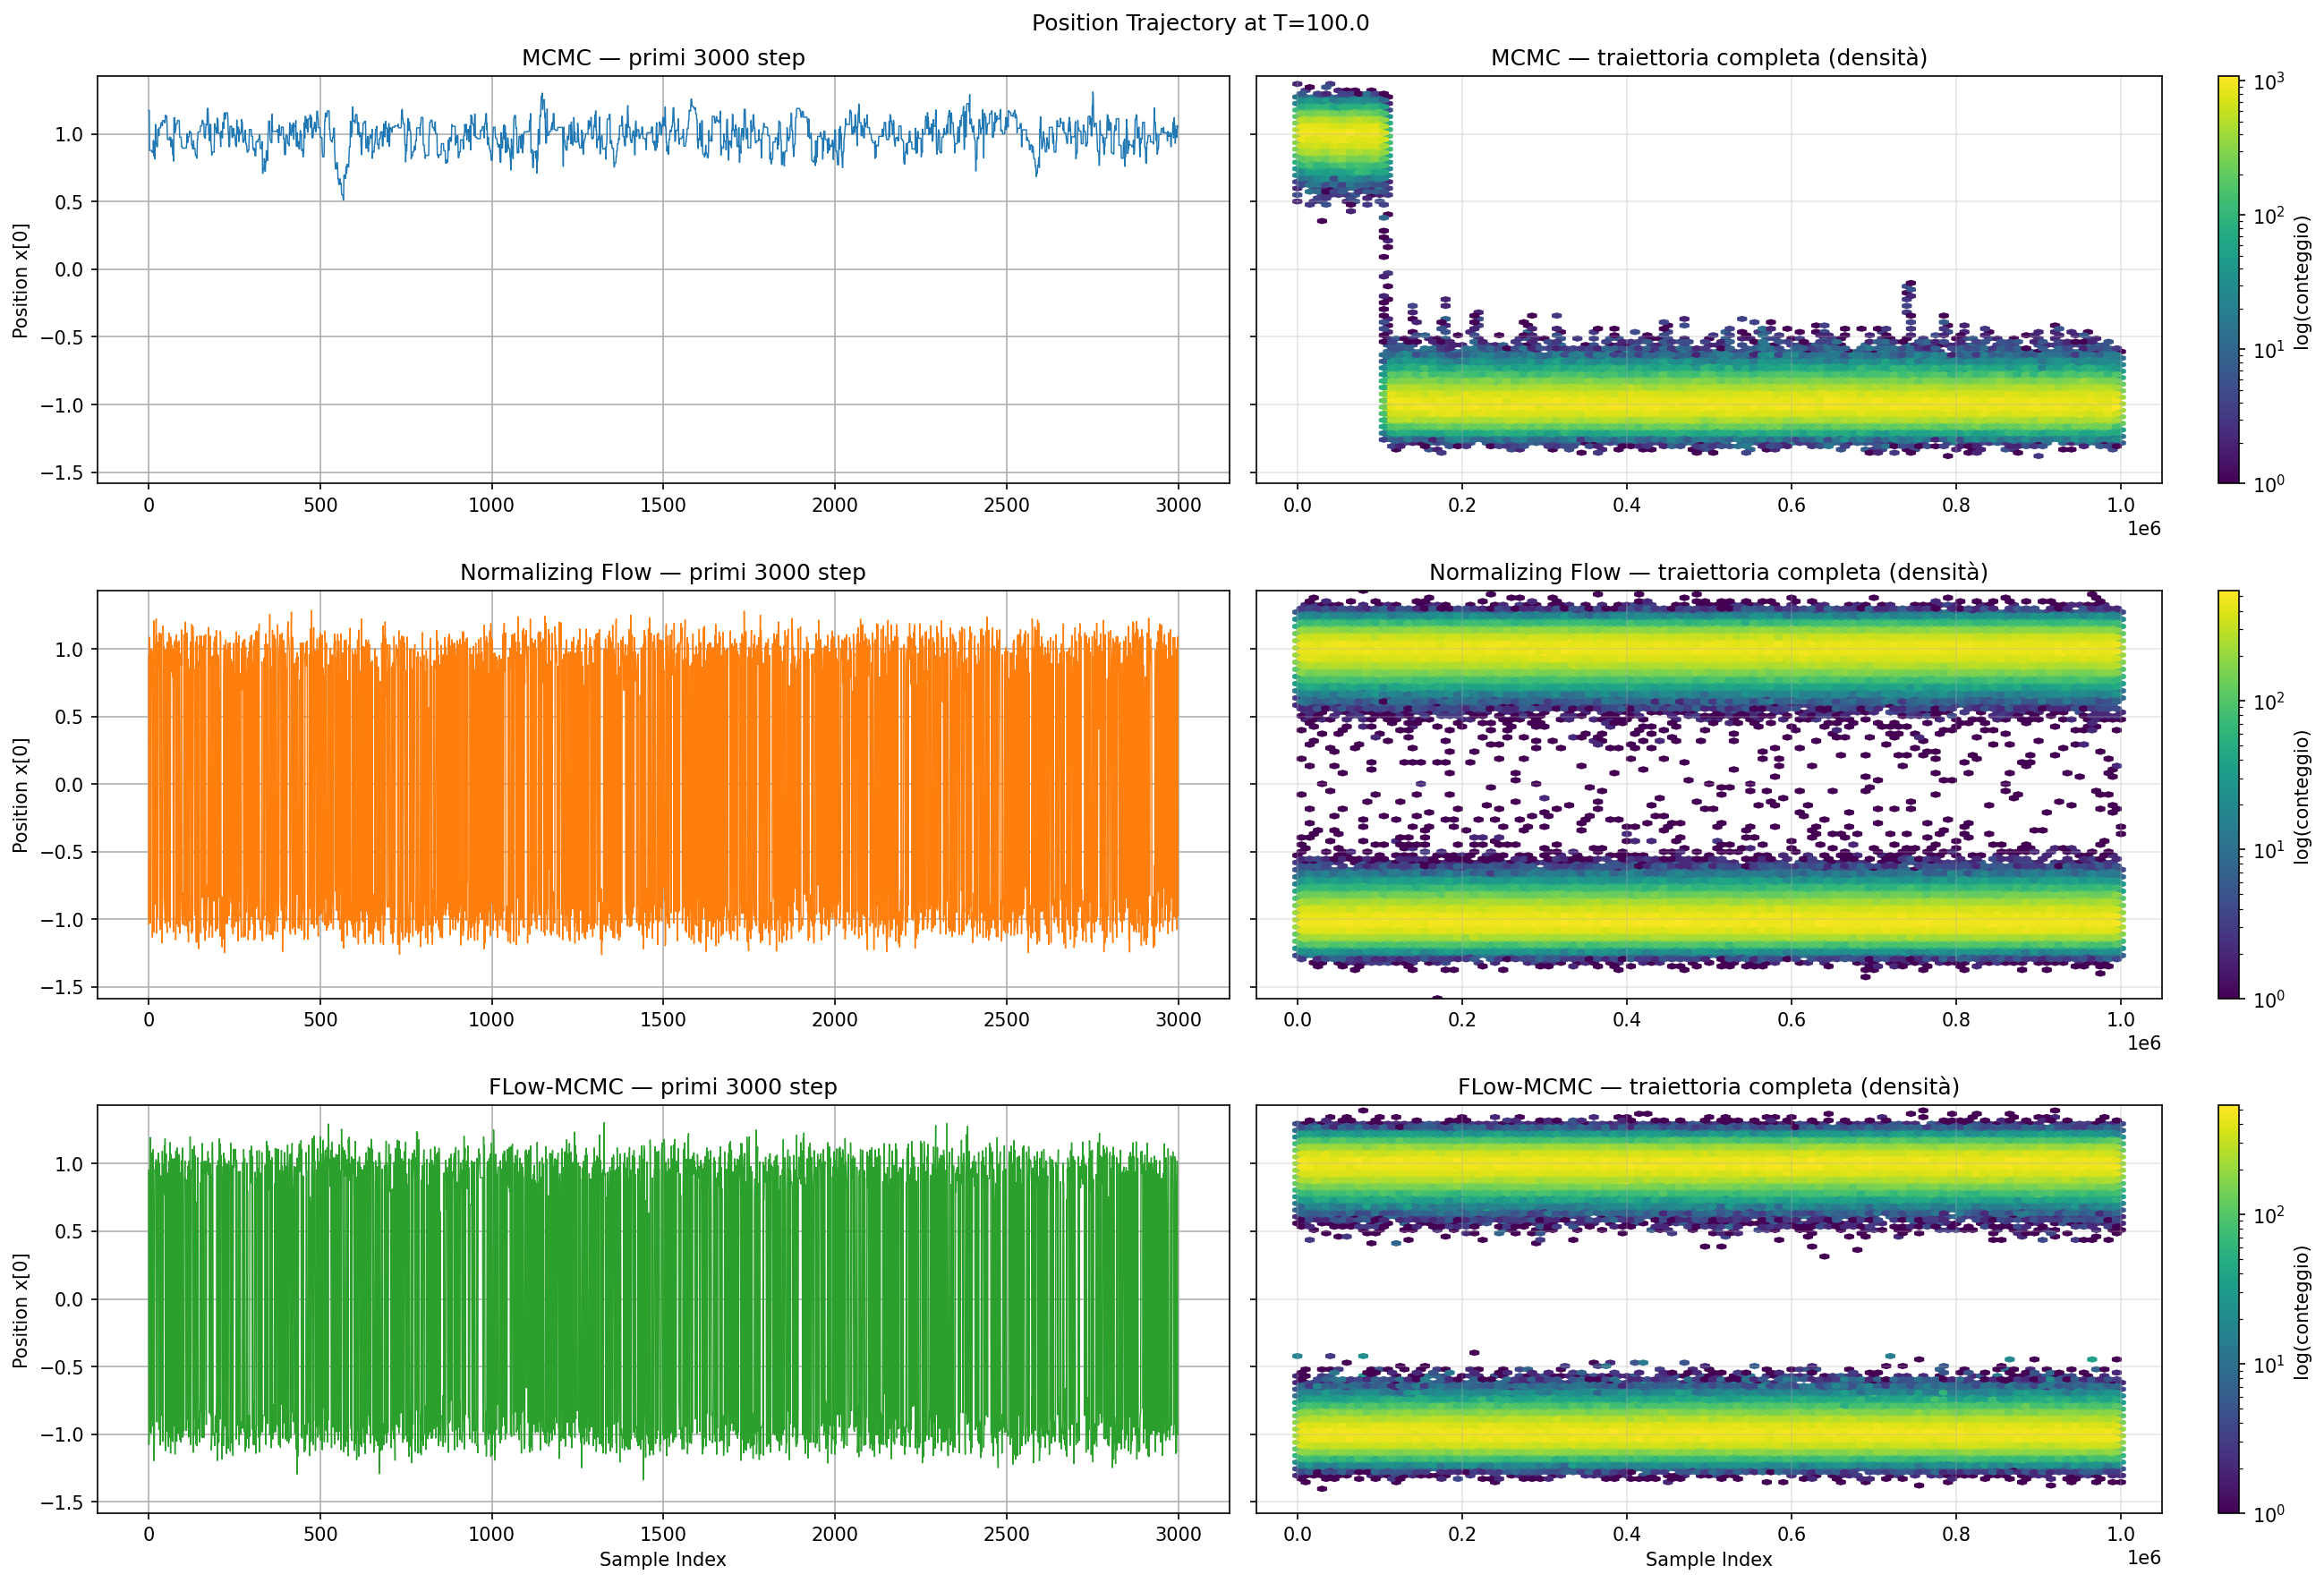
\includegraphics[width=\textwidth]{images/x_trajectory_T_100.0.png}
        \caption{Prima}
    \end{subfigure}
    \hfill
    \begin{subfigure}[b]{0.45\textwidth}
        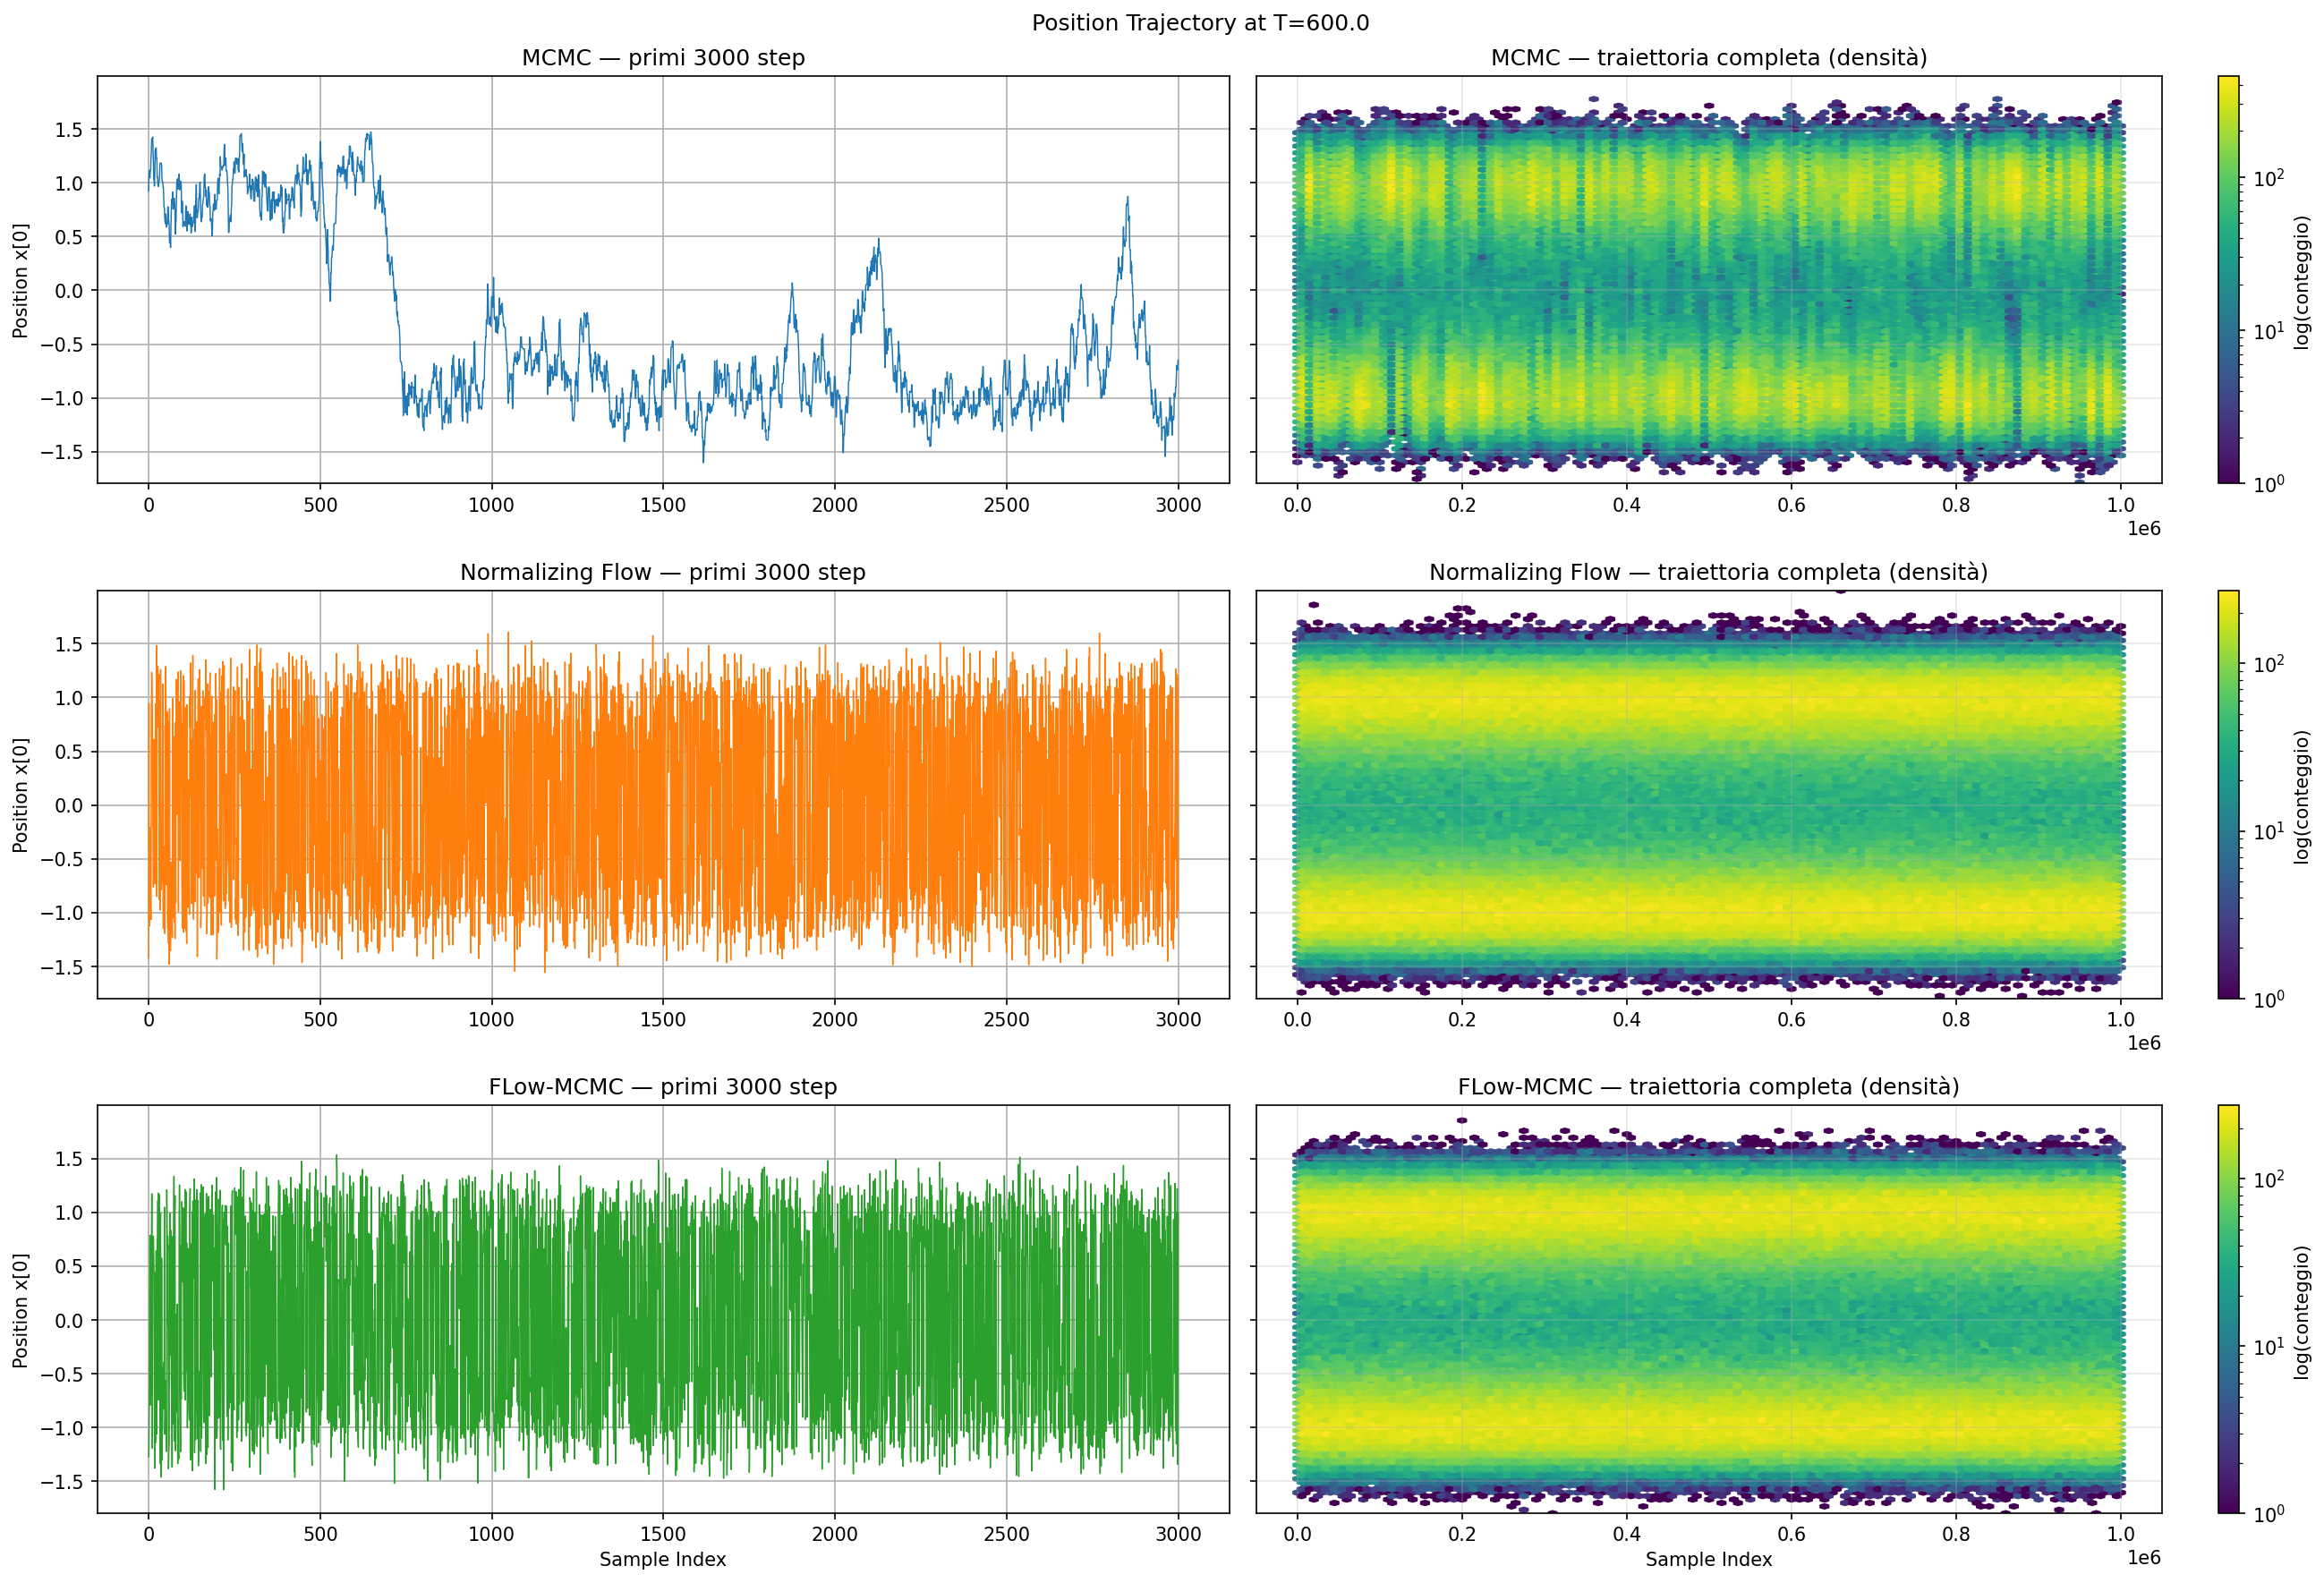
\includegraphics[width=\textwidth]{images/x_trajectory_T_600.0.png}
        \caption{Seconda}
    \end{subfigure}
    
    \vspace{1em}
    
    \begin{subfigure}[b]{0.45\textwidth}
        \centering
        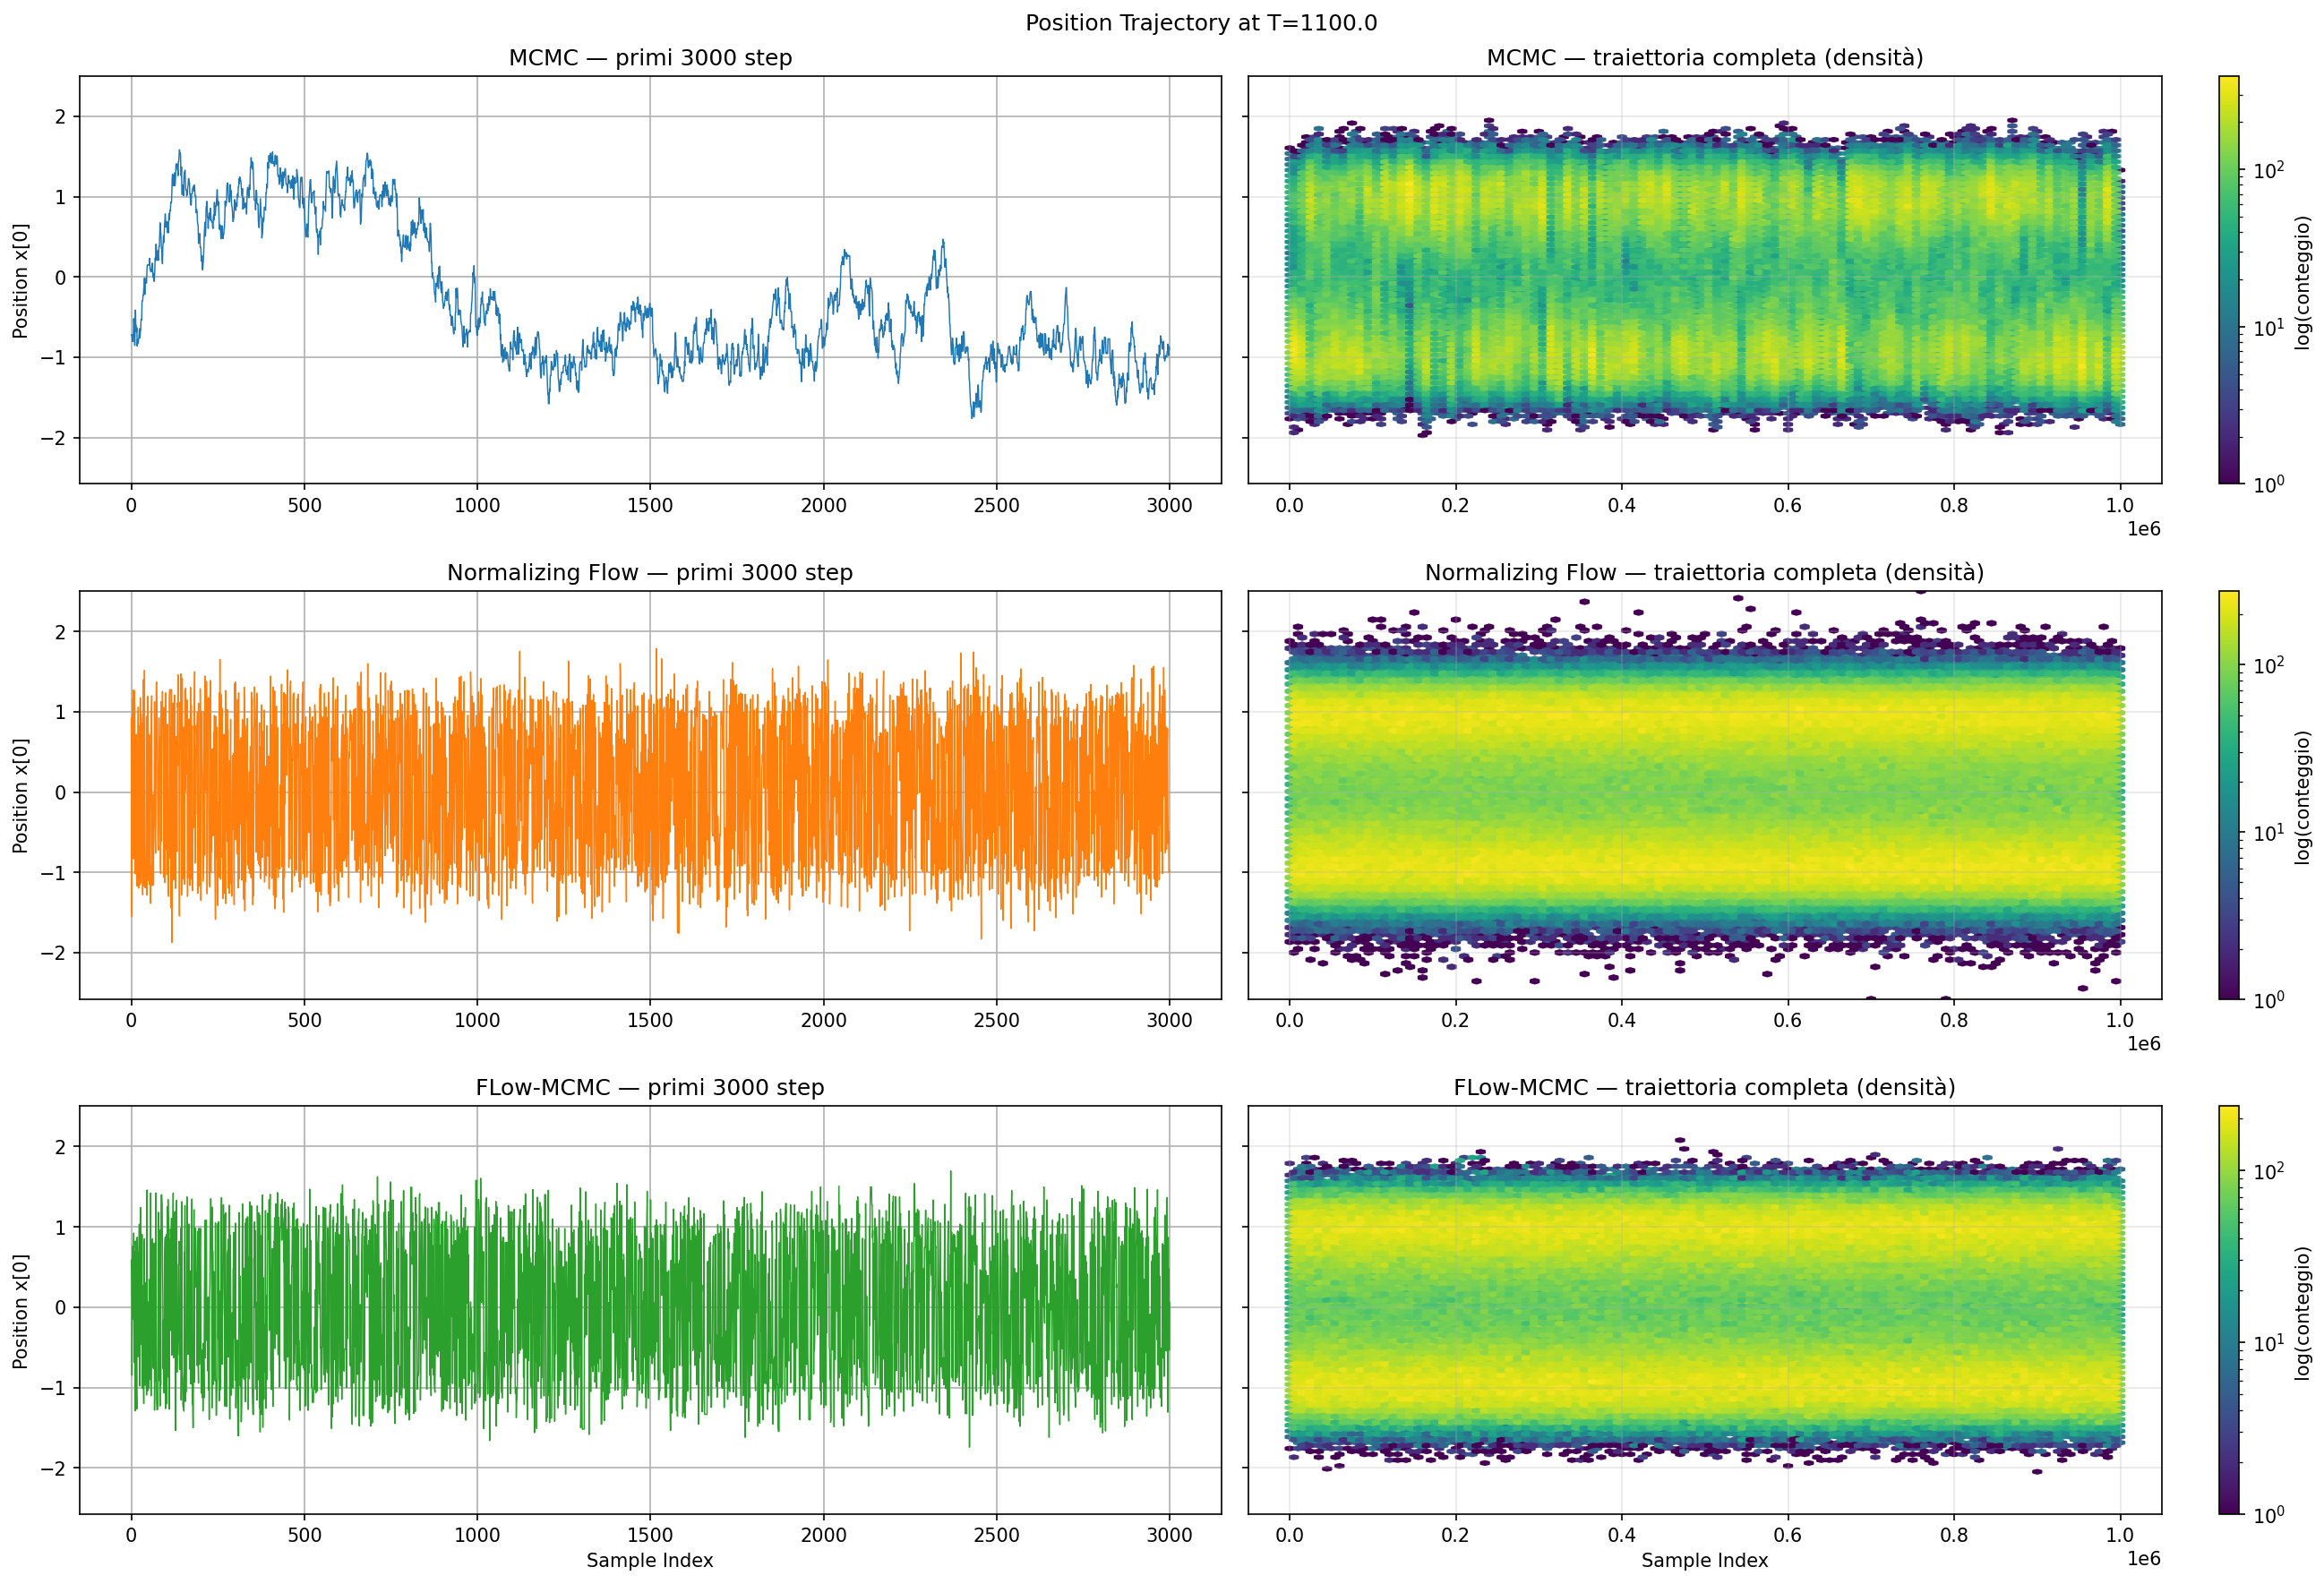
\includegraphics[width=\textwidth]{images/x_trajectory_T_1100.0.png}
        \caption{Terza}
    \end{subfigure}
    \caption{}
\end{figure}


\blankpage
\blankpage
\chapter*{Conclusione}
\addcontentsline{toc}{chapter}{Conclusione}

Nel presente lavoro si è affrontato il problema del campionamento da distribuzioni di Boltzmann multimodali, al fine di stimare le quantità termodinamiche di un sistema a contatto termico con un serbatoio a temperatura ben definita. Si sono confrontate tre strategie concettualmente distinte: il campionamento markoviano locale (MCMC), i Normalizing Flows impiegati come generatori diretti con correzione tramite re-weighting, e lo schema ibrido Flow-MCMC. Il confronto è stato condotto su un sistema di test minimale ma non banale, un potenziale a doppio pozzo affiancato da direzioni armoniche.

I risultati dello studio al variare di dimensione, temperatura e numero di campioni mostrano un quadro coerente. MCMC locale, per costruzione vincolato a esplorare l'intorno immediato dello stato corrente, entra in crisi quando la barriera di potenziale diventa grande rispetto all'energia termica: il tasso di accettazione medio crolla al diminuire della temperatura e all'aumentare della dimensione del sistema, il tempo di autocorrelazione integrato $\tau^{int}$ della coordinata lenta cresce di ordini di grandezza e, nei casi più estremi, la catena rimane intrappolata in una sola delle due buche per l'intera simulazione.

Normalizing Flow e Flow-MCMC non soffrono di questa patologia. Flow-MCMC mantiene un tasso di accettazione medio prossimo a 1 su tutto l'intervallo di temperature esplorato; il tempo di autocorrelazione integrato $\tau^{int}$ e il suo analogo $\tau_{\text{eff}}$ restano vicini al valore ottimale, indipendentemente dalla temperatura. Coerentemente, entrambi i metodi convergono alle stime corrette con un numero di campioni sensibilmente inferiore rispetto a MCMC ed esplorano in modo bilanciato entrambi i pozzi a ogni temperatura considerata. In presenza di distribuzioni multimodali, si conclude dunque che le mosse globali apprese da un Normalizing Flow offrono un vantaggio pratico concreto rispetto al campionamento markoviano locale, sia come motore di campionamento diretto sia come proposta all'interno di uno schema Metropolis-Hastings.

I risultati ottenuti aprono naturalmente a diverse estensioni. Sarebbe auspicabile testare i metodi su potenziali che inducano distribuzioni di Boltzmann più complesse, così da verificare che la robustezza di NF e Flow-MCMC qui osservata si mantenga al crescere della complessità del panorama energetico. Altrettanto importante sarebbe studiare il costo computazionale dei tre metodi, finora confrontati solo in termini di efficienza statistica a parità di campioni generati. Infine, a mio giudizio, sarebbe di estremo interesse applicare direttamente lo schema Flow-MCMC a sistemi fisici realistici, caratterizzati da distribuzioni multimodali e da un numero elevato di gradi di libertà, come proteine, polimeri e materiali ferroelettrici e quantum-paraelettrici come gli ossidi perovskitici.
\blankpage
\appendix

\chapter{Derivazione della distribuzione di Boltzmann}
\label{sec:a_boltzm_der}
Il comportamento del sistema a fissata $T$ è descritto da una distribuzione di probabilità $p (\mathbf{x}, T)$ ottenibile attraverso il principio di massima entropia.
\begin{equation}
    \mathcal{S} = - \int_{\mathbb{R}^D} p (\mathbf{x}, T) \ln(p(\mathbf{x}, T)) d\mathbf{x}
\end{equation}

Per massimizzare l'entropia si utilizza il teorema dei moltiplicatori di Lagrange:

\begin{equation}
    \mathcal{L}[p] = -\int_{\mathbb{R}^D} p \ln p \, d\mathbf{x} - \alpha \left( \int_{\mathbb{R}^D} p \, d\mathbf{x} - 1 \right) - \beta \left( \int_{\mathbb{R}^D} p \, \mathcal{H} \, d\mathbf{x} - \langle E \rangle \right),
\end{equation}

dove $\alpha$ e $\beta$ sono i moltiplicatori di Lagrange associati rispettivamente al vincolo di normalizzazione

\begin{equation}
    \int_{\mathbb{R}^D} p(\mathbf{x}, T) \ d\mathbf{x} = 1 \ ,
\end{equation}

e al vincolo sul valore medio dell'energia

\begin{equation}
    \int_{\mathbb{R}^D} p(\mathbf{x}, T) \, \mathcal{H}(\mathbf{x}) \, d\mathbf{x} = \langle E \rangle .
\end{equation}

La massimizzazione impone $\delta \mathcal{L}/\delta p = 0$ restituendo:

\begin{equation}
    - \ln p(\mathbf{x}, T) - 1 - \alpha - \beta \mathcal{H}(\mathbf{x}) = 0
\end{equation}

che permette di determinare $p (\mathbf{x}, T)$:

\begin{equation}
    p(\mathbf{x}, T) = e^{-1-\alpha} \, e^{-\beta \mathcal{H}(\mathbf{x})}.
\end{equation}

Il moltiplicatore $\alpha$ è fissato dalla condizione di normalizzazione: definendo la \textbf{funzione di partizione}

\begin{equation}
    Z(\beta) = \int_{\mathbb{R}^D} e^{-\beta \mathcal{H}(\mathbf{x})} \ d\mathbf{x},
\end{equation}

si ha $e^{-1-\alpha} = 1/Z(\beta)$, da cui \textbf{la distribuzione di Boltzmann}:

\begin{equation}
    p(\mathbf{x}, T) = \frac{1}{Z(\beta)} e^{-\beta \mathcal{H}(\mathbf{x})}.
\end{equation}

Dove $\beta = 1/(k_B T)$.


\bibliographystyle{unsrt}
\bibliography{Bibliografia}
\addcontentsline{toc}{chapter}{Bibliografia}

\blankpage
\blankpage

\chapter*{Ringraziamenti}
\addcontentsline{toc}{chapter}{Ringraziamenti}

Vorrei ringraziare in primis il mio professore e relatore Cesare Franchini per la passione che mi ha trasmesso per la meccanica statistica e la fisica della materia. Ringrazio il mio correlatore, il dottor Luca Leoni, per la fiducia, la guida e i consigli per il futuro che mi ha dato. 
\vspace{4mm}
\\
Vorrei ringraziare coloro che mi hanno accompagniato e hanno reso questi tre anni di impegno un viaggio che ricorderò col sorriso. Grazie Alice, Bianca, Davide, Giulia, Liang, Lorenzo, Mattia, Nicolò C., Nicolò R., Paolo, Sabrina e Tommy per le serate, i pranzi assieme al parco dietro il dipartimento, le risate durante le lezioni e grazie per le innumerevoli partite a contatto e a carte.
\vspace{4mm}
\\
Ringrazio la mia famiglia: i miei genitori per l'affetto, l'aiuto  e  il sostegno che mi hanno donato durante i periodi più difficili e per avermi dato l'opportunità di fare questo percorso; mio fratello per il mondo che mi ha aperto e mostrato dal liceo all'università.
\vspace{4mm}
\\
Vorrei ringraziare inoltre Maria, Enea ed Alexandra che mi accompagnano con la loro amicizia e il loro affetto fin da quando sono piccolo, tenendo sempre una porta aperta per essere ascoltato.
\vspace{4mm}
\\
Infine voglio ringraziare la mia Sabri che con la sua allegria ha decorato i nostri momenti di spensieratezza e felicità.
Grazie per essermi stata vicina, per avermi sostenuto e capito e per avermi trascinato via dallo studio regalandomi le giornate più belle. 


\end{document}